\batchmode
\makeatletter
\def\input@path{{"E:/Dekstop/ISI_Class_Files/Third Semester/Statistical Computing I/Assignments & Exercises/"}}
\makeatother
\documentclass[11pt,english]{article}\usepackage[]{graphicx}\usepackage[]{xcolor}
% maxwidth is the original width if it is less than linewidth
% otherwise use linewidth (to make sure the graphics do not exceed the margin)
\makeatletter
\def\maxwidth{ %
  \ifdim\Gin@nat@width>\linewidth
    \linewidth
  \else
    \Gin@nat@width
  \fi
}
\makeatother

\definecolor{fgcolor}{rgb}{0.345, 0.345, 0.345}
\newcommand{\hlnum}[1]{\textcolor[rgb]{0.686,0.059,0.569}{#1}}%
\newcommand{\hlstr}[1]{\textcolor[rgb]{0.192,0.494,0.8}{#1}}%
\newcommand{\hlcom}[1]{\textcolor[rgb]{0.678,0.584,0.686}{\textit{#1}}}%
\newcommand{\hlopt}[1]{\textcolor[rgb]{0,0,0}{#1}}%
\newcommand{\hlstd}[1]{\textcolor[rgb]{0.345,0.345,0.345}{#1}}%
\newcommand{\hlkwa}[1]{\textcolor[rgb]{0.161,0.373,0.58}{\textbf{#1}}}%
\newcommand{\hlkwb}[1]{\textcolor[rgb]{0.69,0.353,0.396}{#1}}%
\newcommand{\hlkwc}[1]{\textcolor[rgb]{0.333,0.667,0.333}{#1}}%
\newcommand{\hlkwd}[1]{\textcolor[rgb]{0.737,0.353,0.396}{\textbf{#1}}}%
\let\hlipl\hlkwb

\usepackage{framed}
\makeatletter
\newenvironment{kframe}{%
 \def\at@end@of@kframe{}%
 \ifinner\ifhmode%
  \def\at@end@of@kframe{\end{minipage}}%
  \begin{minipage}{\columnwidth}%
 \fi\fi%
 \def\FrameCommand##1{\hskip\@totalleftmargin \hskip-\fboxsep
 \colorbox{shadecolor}{##1}\hskip-\fboxsep
     % There is no \\@totalrightmargin, so:
     \hskip-\linewidth \hskip-\@totalleftmargin \hskip\columnwidth}%
 \MakeFramed {\advance\hsize-\width
   \@totalleftmargin\z@ \linewidth\hsize
   \@setminipage}}%
 {\par\unskip\endMakeFramed%
 \at@end@of@kframe}
\makeatother

\definecolor{shadecolor}{rgb}{.97, .97, .97}
\definecolor{messagecolor}{rgb}{0, 0, 0}
\definecolor{warningcolor}{rgb}{1, 0, 1}
\definecolor{errorcolor}{rgb}{1, 0, 0}
\newenvironment{knitrout}{}{} % an empty environment to be redefined in TeX

\usepackage{alltt}
\usepackage{lmodern}
\renewcommand{\sfdefault}{lmss}
\renewcommand{\ttdefault}{lmtt}
\renewcommand{\familydefault}{\rmdefault}
\usepackage[T1]{fontenc}
\usepackage[latin9]{inputenc}
\usepackage{geometry}
\geometry{verbose,tmargin=2cm,bmargin=2cm,lmargin=2.5cm,rmargin=2.5cm,headheight=2.5cm,headsep=2.5cm,footskip=2.5cm}
\usepackage{amsmath}
\usepackage{amsthm}

\makeatletter
\@ifundefined{date}{}{\date{}}
\makeatother

\usepackage{babel}
\IfFileExists{upquote.sty}{\usepackage{upquote}}{}
\begin{document}
\title{Statistical Computing I\\
Instructor : Prof. Sourabh Bhattacharya}
\author{Student Name : Spandan Ghoshal\\
Roll : MD2124}
\maketitle

\subsection*{Introduction}

To know whether these estimates are more or less consistent or not
(ergodicity) we plot the cumulative means of these posterior samples.

The Space Shuttle Challenger exploded 73 second after liftoff on January
28th, 1986. The disaster claimed the lives of all seven astronauts
on board, including school teacher Christa McAuliffe.1 The details
surrounding this disaster were very involved. The main concern of
engineers in launching the Challenger was the evidence that the large
O-rings sealing the several sections of the boosters could fail in
cold temperatures.

In this analysis we mainly use the data from previous launches to
get an idea about how the O-rings faliures are associated with covariates
such as surrounding environment temperature and pressure. 

\subsection*{Exploratory Data Analysis}

We first plot, the responses with individual covariates to get idea
about their effects.
\begin{center}
\begin{knitrout}
\definecolor{shadecolor}{rgb}{0.969, 0.969, 0.969}\color{fgcolor}\begin{kframe}
\begin{alltt}
\hlkwd{library}\hlstd{(alr4)}
\hlkwd{library}\hlstd{(ggplot2)}
\hlkwd{library}\hlstd{(glmnet)}

\hlcom{# Data loading}
\hlstd{Datas} \hlkwb{<-} \hlstd{Challeng}
\hlstd{Datas} \hlkwb{<-} \hlstd{Datas[,}\hlnum{1}\hlopt{:}\hlnum{3}\hlstd{]}
\hlkwd{rownames}\hlstd{(Datas)} \hlkwb{<-} \hlkwa{NULL}

\hlstd{normalize} \hlkwb{<-} \hlkwa{function}\hlstd{(}\hlkwc{x}\hlstd{)}
\hlstd{\{}
  \hlkwd{return}\hlstd{((x}\hlopt{-}\hlkwd{mean}\hlstd{(x))}\hlopt{/}\hlkwd{sd}\hlstd{(x))}
\hlstd{\}}


\hlstd{Datas} \hlkwb{<-} \hlkwd{data.frame}\hlstd{(}\hlkwd{lapply}\hlstd{(Datas[,}\hlkwd{c}\hlstd{(}\hlnum{1}\hlstd{,}\hlnum{2}\hlstd{)], normalize),Datas}\hlopt{$}\hlstd{fail)}
\hlstd{Datas}\hlopt{$}\hlstd{Datas.fail[}\hlkwd{which}\hlstd{(Datas}\hlopt{$}\hlstd{Datas.fail} \hlopt{==} \hlnum{2}\hlstd{)]} \hlkwb{<-} \hlnum{1}
\hlcom{# EDA}
\hlkwd{ggplot}\hlstd{(Datas,} \hlkwd{aes}\hlstd{(}\hlkwc{y}\hlstd{=temp,} \hlkwc{x}\hlstd{=Datas.fail))} \hlopt{+}
\hlkwd{geom_jitter}\hlstd{(}\hlkwd{aes}\hlstd{(}\hlkwc{colour}\hlstd{=}\hlkwd{as.factor}\hlstd{(Datas.fail)),}\hlkwc{width} \hlstd{=} \hlnum{0.1}\hlstd{)}
\end{alltt}
\end{kframe}
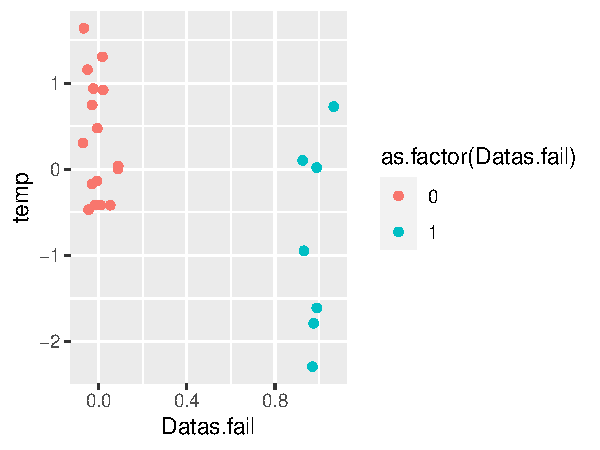
\includegraphics[width=\maxwidth]{figure/unnamed-chunk-1-1} 
\end{knitrout}
\par\end{center}

from the plot of $Y$ versus $x_{1}$ i.e. temperature, we can see
that there is clear negative dependence of temperature with chance
of failure as higher the temperature, lesser $1$ values are observed.
\begin{center}
\begin{knitrout}
\definecolor{shadecolor}{rgb}{0.969, 0.969, 0.969}\color{fgcolor}\begin{kframe}
\begin{alltt}
\hlkwd{ggplot}\hlstd{(Datas,} \hlkwd{aes}\hlstd{(}\hlkwc{y}\hlstd{=pres,} \hlkwc{x}\hlstd{=Datas.fail))} \hlopt{+}
\hlkwd{geom_jitter}\hlstd{(}\hlkwd{aes}\hlstd{(}\hlkwc{colour}\hlstd{=}\hlkwd{as.factor}\hlstd{(Datas.fail)),}\hlkwc{width} \hlstd{=} \hlnum{0.1}\hlstd{)}
\end{alltt}
\end{kframe}
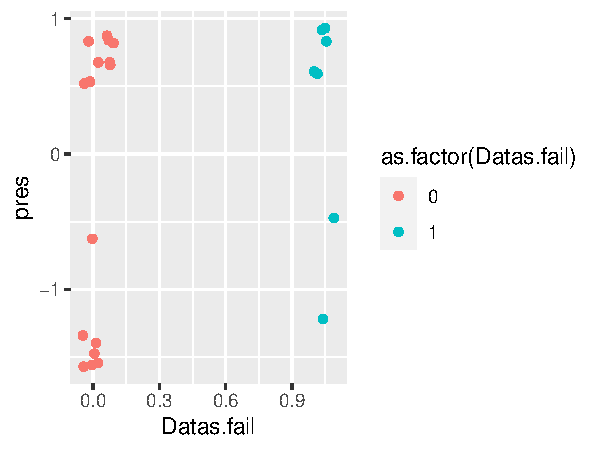
\includegraphics[width=\maxwidth]{figure/unnamed-chunk-2-1} 
\end{knitrout}
\par\end{center}

Whereas, in case of pressure, no such trend is noted as if the failure
doesn't even depend on pressure.
\author{\pagebreak}

\subsection*{Logistic Regression Model}

As the begining, we fit a logistic model with $Y$ as the response
and $x_{1},x_{2}$ as the covariates. Since this is a frequentist
model, for the time being we don't impart any prior information for
the parameters. We just compute their MLEs using \textbf{glm} R package.
Here, are the codes required for that :-
\begin{center}
\begin{knitrout}
\definecolor{shadecolor}{rgb}{0.969, 0.969, 0.969}\color{fgcolor}\begin{kframe}
\begin{alltt}
\hlstd{mod.glm} \hlkwb{<-} \hlkwd{glm}\hlstd{(}\hlkwc{formula} \hlstd{= Datas.fail} \hlopt{~} \hlstd{.,}\hlkwc{family} \hlstd{=} \hlstr{"binomial"}\hlstd{,}\hlkwc{data} \hlstd{= Datas)}
\hlkwd{summary}\hlstd{(mod.glm)}
\end{alltt}
\begin{verbatim}

Call:
glm(formula = Datas.fail ~ ., family = "binomial", data = Datas)

Deviance Residuals: 
    Min       1Q   Median       3Q      Max  
-1.2130  -0.6089  -0.3870   0.3472   2.0928  

Coefficients:
            Estimate Std. Error z value Pr(>|z|)  
(Intercept)  -1.0543     0.5902  -1.786   0.0740 .
temp         -1.7046     0.7743  -2.201   0.0277 *
pres          0.6728     0.6142   1.095   0.2733  
---
Signif. codes:  0 '***' 0.001 '**' 0.01 '*' 0.05 '.' 0.1 ' ' 1

(Dispersion parameter for binomial family taken to be 1)

    Null deviance: 28.267  on 22  degrees of freedom
Residual deviance: 18.972  on 20  degrees of freedom
AIC: 24.972

Number of Fisher Scoring iterations: 5
\end{verbatim}
\end{kframe}
\end{knitrout}
\par\end{center}

Here, from the summary output, we can clearly see that the \textbf{temp
}variable is statistically significant at $5\%$ level whereas \textbf{pres
}is not. This also statistically signifies our suspicion at the begining.
We will use these estimates as initial guesses in the upcoming MCMC
implementations.

Next, to visualize, we plot the fitted logistic model seperately for
the covariates \textbf{temp }and \textbf{pres}.
\begin{center}
\begin{knitrout}
\definecolor{shadecolor}{rgb}{0.969, 0.969, 0.969}\color{fgcolor}\begin{kframe}
\begin{alltt}
\hlkwd{ggplot}\hlstd{( Datas,} \hlkwd{aes}\hlstd{(}\hlkwc{x}\hlstd{=temp,} \hlkwc{y}\hlstd{=Datas.fail))} \hlopt{+}
  \hlkwd{geom_point}\hlstd{()} \hlopt{+}
  \hlkwd{geom_smooth}\hlstd{(}\hlkwc{method} \hlstd{=} \hlstr{"glm"}\hlstd{,}
              \hlkwc{method.args} \hlstd{=} \hlkwd{list}\hlstd{(}\hlkwc{family} \hlstd{=} \hlstr{"binomial"}\hlstd{),}
              \hlkwc{se} \hlstd{=} \hlnum{FALSE}\hlstd{)} \hlopt{+}
\hlkwd{labs}\hlstd{(}\hlkwc{title} \hlstd{=} \hlstr{"Failure Probability"}\hlstd{,}\hlkwc{x} \hlstd{=} \hlstr{"tempareture"}\hlstd{,}\hlkwc{ylab} \hlstd{=} \hlstr{"Failure"}\hlstd{)}
\end{alltt}
\end{kframe}
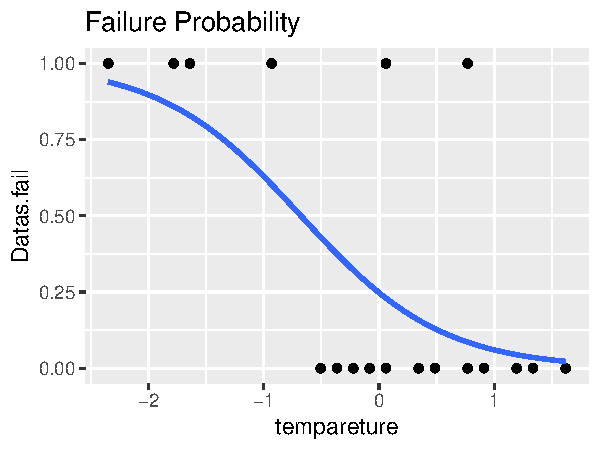
\includegraphics[width=\maxwidth]{figure/unnamed-chunk-4-1} 
\end{knitrout}
\par\end{center}

\begin{center}
\begin{knitrout}
\definecolor{shadecolor}{rgb}{0.969, 0.969, 0.969}\color{fgcolor}\begin{kframe}
\begin{alltt}
\hlcom{# pres}
\hlkwd{ggplot}\hlstd{( Datas,} \hlkwd{aes}\hlstd{(}\hlkwc{x}\hlstd{=pres,} \hlkwc{y}\hlstd{=Datas.fail))} \hlopt{+}
  \hlkwd{geom_point}\hlstd{()} \hlopt{+}
  \hlkwd{geom_smooth}\hlstd{(}\hlkwc{method} \hlstd{=} \hlstr{"glm"}\hlstd{,}
              \hlkwc{method.args} \hlstd{=} \hlkwd{list}\hlstd{(}\hlkwc{family} \hlstd{=} \hlstr{"binomial"}\hlstd{),}
              \hlkwc{se} \hlstd{=} \hlnum{FALSE}\hlstd{)} \hlopt{+}
\hlkwd{labs}\hlstd{(}\hlkwc{title} \hlstd{=} \hlstr{"Failure Probability"}\hlstd{,}\hlkwc{x} \hlstd{=} \hlstr{"pressure"}\hlstd{,}\hlkwc{ylab} \hlstd{=} \hlstr{"Failure"}\hlstd{)}
\end{alltt}
\end{kframe}
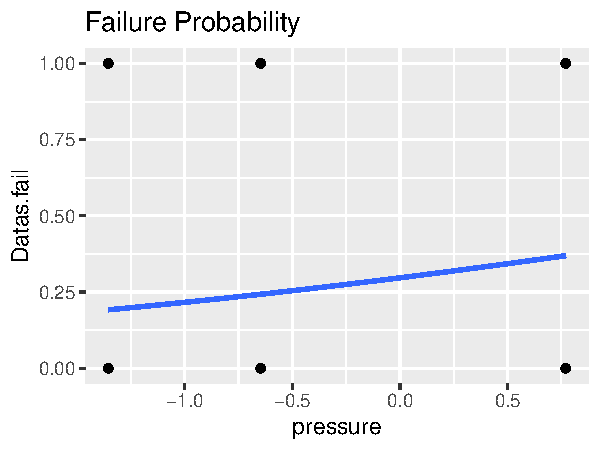
\includegraphics[width=\maxwidth]{figure/unnamed-chunk-5-1} 
\end{knitrout}
\par\end{center}
\author{\pagebreak}

\section*{Bayesian Model 1}

\subsection*{Bayesian Logistic Model 1}

After the frequentist exploration, now we move on to the Bayesian
paradigm. We write the logistic model as :-
\[
P\left(Y_{i}=1|x_{i}\right)=\frac{e^{\beta_{0}+\beta_{1}x_{1i}+\beta_{2}x_{2i}}}{1+e^{\beta_{0}+\beta_{1}x_{1i}+\beta_{2}x_{2i}}}=\pi_{i},i=1,\dots,n
\]

where $x_{1}$ and $x_{2}$ are the normalized variables temperature
and pressure during the launch and $Y$ represents the indicator variable
whether any of the O-rings failed or not.

We consider both the variables $x_{1}$ and $x_{2}$ to be centered
and scaled mainly because of computation issues with the logit link
function. Obviously we can obtain the coefficients in terms of original
variables easily.

The likelihood function of $\boldsymbol{\beta}$ given the observed
data $\boldsymbol{y,X}$ can be written as :-
\begin{align*}
f\left(y_{i}|\boldsymbol{\beta},x_{i}\right) & =\pi_{i}^{y_{i}}\left(1-\pi_{i}\right)^{1-y_{i}}\\
 & =\left[\frac{e^{\beta_{0}+\beta_{1}x_{1i}+\beta_{2}x_{2i}}}{1+e^{\beta_{0}+\beta_{1}x_{1i}+\beta_{2}x_{2i}}}\right]^{y_{i}}\left[\frac{1}{1+e^{\beta_{0}+\beta_{1}x_{1i}+\beta_{2}x_{2i}}}\right]^{1-y_{i}}
\end{align*}

now, if we assume diffused normal prior for $\boldsymbol{\beta}\sim N_{3}\left(\boldsymbol{0},\lambda^{-1}\boldsymbol{I}_{3}\right)$
for small value of $\lambda$ as we don't consider any specific information
to be imparted in the prior :-
\[
\pi\left(\boldsymbol{\beta}\right)\propto\exp\left(-\frac{\lambda}{2}\boldsymbol{\beta}^{T}\boldsymbol{\beta}\right)
\]

Hence, the posterior of $\boldsymbol{\beta}$ can be written as :-
\begin{align*}
\pi\left(\boldsymbol{\beta}|\boldsymbol{x},\boldsymbol{y}\right) & \propto\pi\left(\boldsymbol{\beta}\right)f\left(\boldsymbol{y}|\boldsymbol{\beta},\boldsymbol{x}\right)\\
 & \propto\exp\left(-\frac{\lambda}{2}\boldsymbol{\beta}^{T}\boldsymbol{\beta}\right)\prod_{i=1}^{n}\left[\frac{e^{\beta_{0}+\beta_{1}x_{1i}+\beta_{2}x_{2i}}}{1+e^{\beta_{0}+\beta_{1}x_{1i}+\beta_{2}x_{2i}}}\right]^{y_{i}}\left[\frac{1}{1+e^{\beta_{0}+\beta_{1}x_{1i}+\beta_{2}x_{2i}}}\right]^{1-y_{i}}\\
 & \propto\exp\left(-\frac{\lambda}{2}\boldsymbol{\beta}^{T}\boldsymbol{\beta}\right)\prod\limits _{i=1}^{n}\left[\frac{e^{y_{i}\boldsymbol{\beta}^{T}\boldsymbol{x_{i}}}}{1+e^{\boldsymbol{\beta}^{T}\boldsymbol{x_{i}}}}\right]\left(=\widetilde{p}\left(\boldsymbol{\beta}\right)\right)
\end{align*}

Now, in order to draw samples from this posterior distribution of
$\boldsymbol{\beta}$, we use the following MCMC algorithm.
\begin{itemize}
\item We have to draw samples from the posterior distribution of $\boldsymbol{\beta}$
which can be written as $p\left(\boldsymbol{\beta}\right)=\frac{\widetilde{p}\left(\boldsymbol{\beta}\right)}{Z_{p}}$
where, $Z_{p}$ denotes the intractible normalizing constant and $\widetilde{p}\left(\boldsymbol{\beta}\right)$
denotes the part that is easily computable.
\item Now, we select our proposal distribution as $q\left(\boldsymbol{\beta}|\boldsymbol{\beta}^{\left(\tau\right)}\right)$
where $\boldsymbol{\beta}^{\left(\tau\right)}$is the current iterate
of $\boldsymbol{\beta}$. For implementing the basic Markov Chain
Monte Carlo, we choose, $q\left(\right)$ to be a symmetric distribution
i.e., 
\[
q\left(\boldsymbol{\beta}|\boldsymbol{\beta}^{\left(\tau\right)}\right)\sim N_{3}\left(\boldsymbol{\beta}^{\left(\tau\right)},\Sigma\right)
\]
 which is a trivariate normal density with mean $\boldsymbol{\beta}^{\left(\tau\right)}$
and variance covariance matrix $\Sigma$. We take $\Sigma=\text{diag}\left(\sigma_{1},\sigma_{2},\sigma_{3}\right)$
where $\sigma_{i}$ are chosen in such a manner that the target distribution
is neither explored too slowly such that it gets stuck in a mode even
if the posterior is multimodal, nor too large that the acceptance
probbility becomes too low.
\item Finally, in an iteration $\tau$, where current value is $\boldsymbol{\beta}^{\left(\tau\right)}$,
we select a new value $\boldsymbol{\beta}^{*}$ if $u<A\left(\boldsymbol{\beta}^{*},\boldsymbol{\beta}^{\left(\tau\right)}\right)$
where : 
\begin{itemize}
\item $u\sim U\left(0,1\right)$ is an uniform random sample.
\item $A\left(\boldsymbol{\beta}^{*},\boldsymbol{\beta}^{\left(\tau\right)}\right)$
is the acceptance probability defined as $A\left(\boldsymbol{\beta}^{*},\boldsymbol{\beta}^{\left(\tau\right)}\right)=\min\left(1,\frac{\widetilde{p}\left(\boldsymbol{\beta}^{*}\right)}{\widetilde{p}\left(\boldsymbol{\beta}^{\left(\tau\right)}\right)}\right)$. 
\item then we set $\boldsymbol{\beta}^{\left(\tau+1\right)}=\boldsymbol{\beta}^{*}$
and proceed.
\end{itemize}
\item Otherwise also we set $\boldsymbol{\beta}^{\left(\tau+1\right)}=\boldsymbol{\beta}^{\left(\tau\right)}$
and draw samples from proposal distribution $q\left(\boldsymbol{\beta}|\boldsymbol{\beta}^{\left(\tau+1\right)}\right)$.
\end{itemize}
We draw $B=5\times10^{4}$ many samples from the posterior distribution
using MCMC algorithm devised above and burn the first $10\%$ samples
also use a thinning gap of $5$ to avoid significant correlations
between the observations. Here are the relevant R codes for the analysis
:-

\begin{knitrout}
\definecolor{shadecolor}{rgb}{0.969, 0.969, 0.969}\color{fgcolor}\begin{kframe}
\begin{alltt}
\hlstd{likelihood1} \hlkwb{<-} \hlkwa{function}\hlstd{(}\hlkwc{X}\hlstd{,}\hlkwc{y}\hlstd{,}\hlkwc{beta}\hlstd{,}\hlkwc{lambda} \hlstd{=} \hlnum{0.01}\hlstd{,}\hlkwc{M} \hlstd{=} \hlnum{100}\hlstd{)}
\hlstd{\{}
  \hlstd{beta} \hlkwb{=} \hlkwd{matrix}\hlstd{(beta,}\hlkwc{nrow} \hlstd{=} \hlnum{1}\hlstd{)}
  \hlstd{a} \hlkwb{=} \hlkwd{exp}\hlstd{(}\hlopt{-}\hlstd{(lambda}\hlopt{/}\hlnum{2}\hlstd{)}\hlopt{*}\hlstd{beta}\hlopt\hlkwd{t}\hlstd{(beta))}
  \hlstd{b} \hlkwb{=} \hlkwd{exp}\hlstd{(y}\hlopt{*}\hlstd{(beta}\hlopt\hlkwd{t}\hlstd{(X)))}
  \hlstd{c} \hlkwb{=} \hlkwd{exp}\hlstd{(beta}\hlopt\hlkwd{t}\hlstd{(X))}
  \hlkwd{return}\hlstd{(M}\hlopt{*}\hlstd{a}\hlopt{*}\hlkwd{prod}\hlstd{(b}\hlopt{/}\hlstd{(}\hlnum{1}\hlopt{+}\hlstd{c)))}
\hlstd{\}}

\hlstd{MCMC.Sampler1} \hlkwb{<-} \hlkwa{function}\hlstd{(}\hlkwc{X}\hlstd{,}\hlkwc{y}\hlstd{,}\hlkwc{beta0}\hlstd{,}\hlkwc{B}\hlstd{,}\hlkwc{sg} \hlstd{=} \hlkwd{c}\hlstd{(}\hlnum{1}\hlstd{,}\hlnum{1}\hlstd{,}\hlnum{1}\hlstd{),}\hlkwc{showprogress} \hlstd{=} \hlnum{TRUE}\hlstd{,}\hlkwc{...}\hlstd{)}
\hlstd{\{}
  \hlstd{X} \hlkwb{=} \hlkwd{cbind}\hlstd{(}\hlkwd{rep}\hlstd{(}\hlnum{1}\hlstd{,}\hlkwd{nrow}\hlstd{(X)),X)}
  \hlstd{beta0} \hlkwb{=} \hlkwd{matrix}\hlstd{(beta0,}\hlkwc{nrow} \hlstd{=} \hlnum{1}\hlstd{)}
  \hlstd{post.sample} \hlkwb{=} \hlkwd{c}\hlstd{(}\hlnum{0}\hlstd{,}\hlnum{0}\hlstd{,}\hlnum{0}\hlstd{)}
  \hlstd{beta1} \hlkwb{=} \hlstd{beta0}
  \hlstd{beta2} \hlkwb{=} \hlkwd{matrix}\hlstd{(}\hlkwd{c}\hlstd{(}\hlnum{0}\hlstd{,}\hlnum{0}\hlstd{,}\hlnum{0}\hlstd{),}\hlkwc{nrow} \hlstd{=} \hlnum{1}\hlstd{)}
  \hlstd{prog} \hlkwb{=} \hlkwd{txtProgressBar}\hlstd{(}\hlkwc{max} \hlstd{= B,}\hlkwc{style} \hlstd{=} \hlnum{3}\hlstd{)}
  \hlkwa{for}\hlstd{(i} \hlkwa{in} \hlnum{1}\hlopt{:}\hlstd{B)}
  \hlstd{\{}
    \hlstd{beta2[}\hlnum{1}\hlstd{]} \hlkwb{=} \hlstd{beta1[}\hlnum{1}\hlstd{]} \hlopt{+} \hlkwd{rnorm}\hlstd{(}\hlnum{1}\hlstd{,}\hlnum{0}\hlstd{,sg[}\hlnum{1}\hlstd{])}
    \hlstd{beta2[}\hlnum{2}\hlstd{]} \hlkwb{=} \hlstd{beta1[}\hlnum{2}\hlstd{]} \hlopt{+} \hlkwd{rnorm}\hlstd{(}\hlnum{1}\hlstd{,}\hlnum{0}\hlstd{,sg[}\hlnum{2}\hlstd{])}
    \hlstd{beta2[}\hlnum{3}\hlstd{]} \hlkwb{=} \hlstd{beta1[}\hlnum{3}\hlstd{]} \hlopt{+} \hlkwd{rnorm}\hlstd{(}\hlnum{1}\hlstd{,}\hlnum{0}\hlstd{,sg[}\hlnum{3}\hlstd{])}
    \hlstd{ratio} \hlkwb{=} \hlkwd{likelihood1}\hlstd{(X,y,}\hlkwc{beta} \hlstd{= beta2,...)}\hlopt{/}\hlkwd{likelihood1}\hlstd{(X,y,beta1,...)}
    \hlstd{unif} \hlkwb{=} \hlkwd{runif}\hlstd{(}\hlnum{1}\hlstd{)}
    \hlkwa{if}\hlstd{(unif} \hlopt{<=} \hlkwd{min}\hlstd{(}\hlnum{1}\hlstd{,ratio)) beta1}\hlkwb{=}\hlstd{beta2}
    \hlstd{post.sample} \hlkwb{=} \hlkwd{rbind}\hlstd{(post.sample,beta1)}
    \hlkwa{if}\hlstd{(showprogress)} \hlkwd{setTxtProgressBar}\hlstd{(}\hlkwc{pb} \hlstd{= prog,}\hlkwc{value} \hlstd{= i)}
  \hlstd{\}}
  \hlkwd{close}\hlstd{(prog)}
  \hlkwd{return}\hlstd{(post.sample)}
\hlstd{\}}
\end{alltt}
\end{kframe}
\end{knitrout}

Using this manual function we draw the stated number of posterior
samples and make inference from them 

\begin{knitrout}
\definecolor{shadecolor}{rgb}{0.969, 0.969, 0.969}\color{fgcolor}\begin{kframe}
\begin{alltt}
\hlcom{# MCMC parameters}
\hlstd{B} \hlkwb{=} \hlnum{10}\hlopt{^}\hlnum{5}
\hlstd{n.thin} \hlkwb{=} \hlnum{5}

\hlcom{# Running the MCMC sampler}
\hlstd{Post.Sample1} \hlkwb{=} \hlkwd{MCMC.Sampler1}\hlstd{(}\hlkwc{X} \hlstd{= Datas[,}\hlnum{1}\hlopt{:}\hlnum{2}\hlstd{],}\hlkwc{y} \hlstd{= Datas}\hlopt{$}\hlstd{Datas.fail,}\hlkwc{beta0} \hlstd{=}
\hlkwd{c}\hlstd{(mod.glm}\hlopt{$}\hlstd{coefficients[}\hlnum{1}\hlstd{],mod.glm}\hlopt{$}\hlstd{coefficients[}\hlnum{2}\hlstd{],mod.glm}\hlopt{$}\hlstd{coefficients[}\hlnum{3}\hlstd{]),B,}
\hlkwc{sg} \hlstd{=} \hlkwd{c}\hlstd{(}\hlnum{3}\hlstd{,}\hlnum{3}\hlstd{,}\hlnum{3}\hlstd{),}\hlkwc{showprogress} \hlstd{=} \hlnum{FALSE}\hlstd{,}\hlkwc{lambda}\hlstd{=}\hlnum{0.001}\hlstd{)}
\end{alltt}
\begin{verbatim}

  |                                                                            
  |                                                                      |   0%
\end{verbatim}
\begin{alltt}
\hlstd{Post.Sample1} \hlkwb{=} \hlstd{(Post.Sample1)[}\hlopt{-}\hlstd{(}\hlnum{1}\hlopt{:}\hlstd{(B}\hlopt{/}\hlnum{10}\hlstd{)),]}
\hlstd{n.length} \hlkwb{=} \hlkwd{nrow}\hlstd{(Post.Sample1)}
\hlstd{batch.size} \hlkwb{=} \hlkwd{floor}\hlstd{(n.length}\hlopt{/}\hlstd{n.thin)}
\hlstd{Post.Sample1} \hlkwb{=} \hlstd{Post.Sample1[n.thin}\hlopt{*}\hlstd{(}\hlnum{1}\hlopt{:}\hlstd{batch.size),]}
\hlstd{Post.Samp1} \hlkwb{=} \hlkwd{data.frame}\hlstd{(Post.Sample1)}
\hlkwd{names}\hlstd{(Post.Samp1)} \hlkwb{<-} \hlkwd{c}\hlstd{(}\hlstr{'b0'}\hlstd{,}\hlstr{'b1'}\hlstd{,}\hlstr{'b2'}\hlstd{)}
\end{alltt}
\end{kframe}
\end{knitrout}

Now, using the generated posterior samples, we plot the posterior
densities of $\boldsymbol{\beta}$ individually. 
\begin{center}
\begin{knitrout}
\definecolor{shadecolor}{rgb}{0.969, 0.969, 0.969}\color{fgcolor}\begin{kframe}
\begin{alltt}
\hlcom{# Posterior distributions of beta0,beta1}
\hlkwd{ggplot}\hlstd{(}\hlkwc{data} \hlstd{= Post.Samp1,}\hlkwd{aes}\hlstd{(}\hlkwc{x}\hlstd{=b0))} \hlopt{+}
  \hlkwd{geom_density}\hlstd{(}\hlkwc{fill}\hlstd{=}\hlstr{"#69b3a2"}\hlstd{,} \hlkwc{color}\hlstd{=}\hlstr{"#e9ecef"}\hlstd{,} \hlkwc{alpha}\hlstd{=}\hlnum{0.8}\hlstd{)} \hlopt{+}
    \hlkwd{labs}\hlstd{(}\hlkwc{title} \hlstd{=} \hlkwd{bquote}\hlstd{(}\hlstr{"Density Plot of"} \hlopt{~} \hlstd{beta[}\hlnum{0}\hlstd{]),}\hlkwc{x} \hlstd{=} \hlkwd{bquote}\hlstd{(beta[}\hlnum{0}\hlstd{]))}
\end{alltt}
\end{kframe}
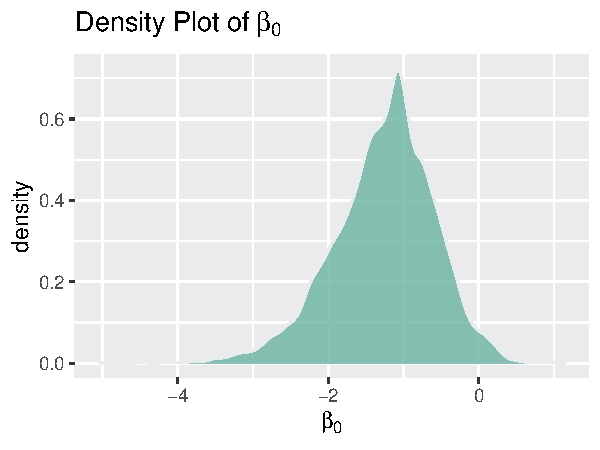
\includegraphics[width=\maxwidth]{figure/unnamed-chunk-8-1} 
\begin{kframe}\begin{alltt}
\hlkwd{ggplot}\hlstd{(}\hlkwc{data} \hlstd{= Post.Samp1,}\hlkwd{aes}\hlstd{(}\hlkwc{x}\hlstd{=b1))} \hlopt{+}
  \hlkwd{geom_density}\hlstd{(}\hlkwc{fill}\hlstd{=}\hlstr{"#69b3a2"}\hlstd{,} \hlkwc{color}\hlstd{=}\hlstr{"#e9ecef"}\hlstd{,} \hlkwc{alpha}\hlstd{=}\hlnum{0.8}\hlstd{)} \hlopt{+}
  \hlkwd{labs}\hlstd{(}\hlkwc{title} \hlstd{=} \hlkwd{bquote}\hlstd{(}\hlstr{"Density Plot of"} \hlopt{~} \hlstd{beta[}\hlnum{1}\hlstd{]),}\hlkwc{x} \hlstd{=} \hlkwd{bquote}\hlstd{(beta[}\hlnum{1}\hlstd{]))}
\end{alltt}
\end{kframe}
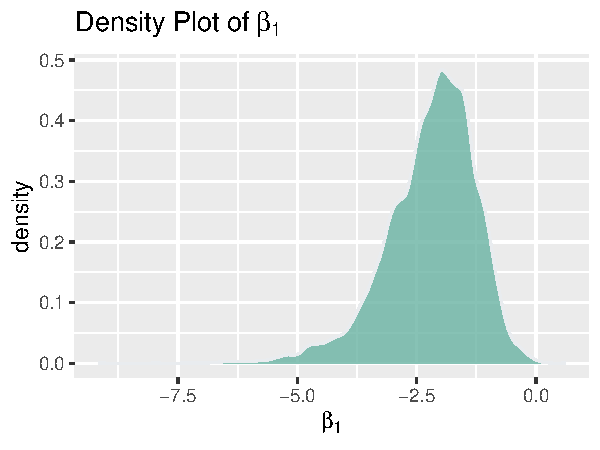
\includegraphics[width=\maxwidth]{figure/unnamed-chunk-8-2} 
\begin{kframe}\begin{alltt}
\hlkwd{ggplot}\hlstd{(}\hlkwc{data} \hlstd{= Post.Samp1,}\hlkwd{aes}\hlstd{(}\hlkwc{x}\hlstd{=b2))} \hlopt{+}
  \hlkwd{geom_density}\hlstd{(}\hlkwc{fill}\hlstd{=}\hlstr{"#69b3a2"}\hlstd{,} \hlkwc{color}\hlstd{=}\hlstr{"#e9ecef"}\hlstd{,} \hlkwc{alpha}\hlstd{=}\hlnum{0.8}\hlstd{)} \hlopt{+}
  \hlkwd{labs}\hlstd{(}\hlkwc{title} \hlstd{=} \hlkwd{bquote}\hlstd{(}\hlstr{"Density Plot of"} \hlopt{~} \hlstd{beta[}\hlnum{2}\hlstd{]),}\hlkwc{x} \hlstd{=} \hlkwd{bquote}\hlstd{(beta[}\hlnum{2}\hlstd{]))}
\end{alltt}
\end{kframe}
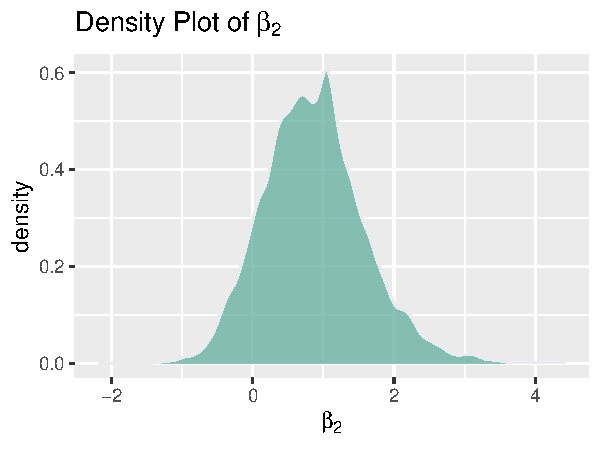
\includegraphics[width=\maxwidth]{figure/unnamed-chunk-8-3} 
\end{knitrout}
\par\end{center}

The posterior means for the three parameters are :-

\begin{knitrout}
\definecolor{shadecolor}{rgb}{0.969, 0.969, 0.969}\color{fgcolor}\begin{kframe}
\begin{alltt}
\hlstd{m1} \hlkwb{=} \hlkwd{apply}\hlstd{(Post.Samp1,} \hlnum{2}\hlstd{, mean)}
\hlstd{m2} \hlkwb{=} \hlstd{mod.glm}\hlopt{$}\hlstd{coefficients}
\hlkwd{data.frame}\hlstd{(}\hlstr{"Posterior.Means"} \hlstd{= m1,}\hlstr{"Logistic.Coef"} \hlstd{= m2)}
\end{alltt}
\begin{verbatim}
   Posterior.Means Logistic.Coef
b0      -1.2623902    -1.0543469
b1      -2.2007295    -1.7045661
b2       0.8659067     0.6728236
\end{verbatim}
\end{kframe}
\end{knitrout}

To know whether these estimates are more or less consistent or not
(ergodicity) we plot the cumulative means of these posterior samples. 
\begin{center}
\begin{knitrout}
\definecolor{shadecolor}{rgb}{0.969, 0.969, 0.969}\color{fgcolor}\begin{kframe}
\begin{alltt}
\hlcom{# plotting the mean cumulatively w.r.t sample size}
\hlstd{b0.mean.cum} \hlkwb{<-} \hlkwd{cumsum}\hlstd{(Post.Samp1}\hlopt{$}\hlstd{b0)}\hlopt{/}\hlstd{(}\hlnum{1}\hlopt{:}\hlkwd{nrow}\hlstd{(Post.Samp1))}
\hlstd{b1.mean.cum} \hlkwb{<-} \hlkwd{cumsum}\hlstd{(Post.Samp1}\hlopt{$}\hlstd{b1)}\hlopt{/}\hlstd{(}\hlnum{1}\hlopt{:}\hlkwd{nrow}\hlstd{(Post.Samp1))}
\hlstd{b2.mean.cum} \hlkwb{<-} \hlkwd{cumsum}\hlstd{(Post.Samp1}\hlopt{$}\hlstd{b2)}\hlopt{/}\hlstd{(}\hlnum{1}\hlopt{:}\hlkwd{nrow}\hlstd{(Post.Samp1))}
\hlcom{# plot of means with increasing sample size}
\hlkwd{plot}\hlstd{(b0.mean.cum,}\hlkwc{type} \hlstd{=} \hlstr{"l"}\hlstd{,}\hlkwc{main} \hlstd{=} \hlkwd{bquote}\hlstd{(}\hlstr{"posterior mean of "} \hlopt{~} \hlstd{beta[}\hlnum{0}\hlstd{]),}
\hlkwc{xlab} \hlstd{=} \hlkwd{bquote}\hlstd{(beta[}\hlnum{0}\hlstd{]),}\hlkwc{ylab} \hlstd{=} \hlstr{"mean"}\hlstd{)}
\end{alltt}
\end{kframe}
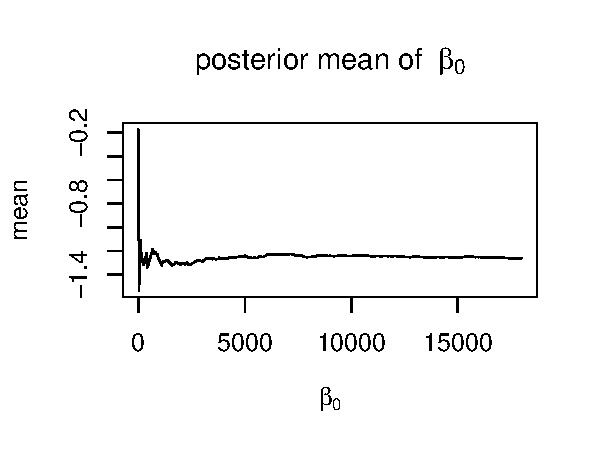
\includegraphics[width=\maxwidth]{figure/unnamed-chunk-10-1} 
\begin{kframe}\begin{alltt}
\hlkwd{plot}\hlstd{(b1.mean.cum,}\hlkwc{type} \hlstd{=} \hlstr{"l"}\hlstd{,}\hlkwc{main} \hlstd{=} \hlkwd{bquote}\hlstd{(}\hlstr{"posterior mean of "} \hlopt{~} \hlstd{beta[}\hlnum{1}\hlstd{]),}
\hlkwc{xlab} \hlstd{=} \hlkwd{bquote}\hlstd{(beta[}\hlnum{1}\hlstd{]),}\hlkwc{ylab} \hlstd{=} \hlstr{"mean"}\hlstd{)}
\end{alltt}
\end{kframe}
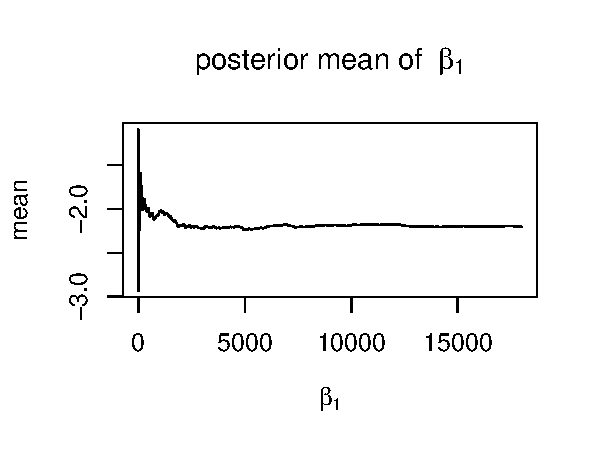
\includegraphics[width=\maxwidth]{figure/unnamed-chunk-10-2} 
\begin{kframe}\begin{alltt}
\hlkwd{plot}\hlstd{(b2.mean.cum,}\hlkwc{type} \hlstd{=} \hlstr{"l"}\hlstd{,}\hlkwc{main} \hlstd{=} \hlkwd{bquote}\hlstd{(}\hlstr{"posterior mean of "} \hlopt{~} \hlstd{beta[}\hlnum{2}\hlstd{]),}
\hlkwc{xlab} \hlstd{=} \hlkwd{bquote}\hlstd{(beta[}\hlnum{2}\hlstd{]),}\hlkwc{ylab} \hlstd{=} \hlstr{"mean"}\hlstd{)}
\end{alltt}
\end{kframe}
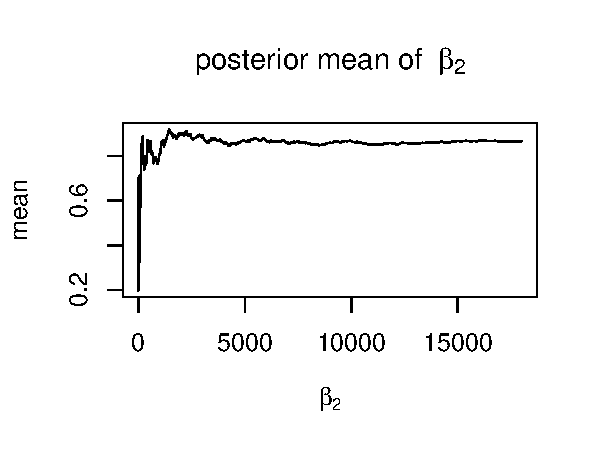
\includegraphics[width=\maxwidth]{figure/unnamed-chunk-10-3} 
\end{knitrout}
\par\end{center}

With increasing sample size, we can see that the mean more or less
gets stabilized indicating their consistency.

Here's another plot which may provide better idea through bivariate
density plots taking two variables at a time where the density is
shown using varying colour density.
\begin{center}
\begin{knitrout}
\definecolor{shadecolor}{rgb}{0.969, 0.969, 0.969}\color{fgcolor}\begin{kframe}
\begin{alltt}
\hlcom{# b0,b1}
\hlkwd{ggplot}\hlstd{(Post.Samp1,} \hlkwd{aes}\hlstd{(}\hlkwc{x} \hlstd{= b0,} \hlkwc{y} \hlstd{= b1,} \hlkwc{fill} \hlstd{= ..level..))} \hlopt{+}
  \hlkwd{stat_density_2d}\hlstd{(}\hlkwc{geom} \hlstd{=} \hlstr{"polygon"}\hlstd{)} \hlopt{+}
\hlkwd{labs}\hlstd{(}\hlkwc{title} \hlstd{=} \hlkwd{bquote}\hlstd{(}\hlstr{"Joint Density of"} \hlopt{~} \hlstd{beta[}\hlnum{0}\hlstd{]} \hlopt{~} \hlstr{"&"} \hlopt{~} \hlstd{beta[}\hlnum{1}\hlstd{]),}
\hlkwc{x} \hlstd{=} \hlkwd{bquote}\hlstd{(beta[}\hlnum{0}\hlstd{]),} \hlkwc{y} \hlstd{=} \hlkwd{bquote}\hlstd{(beta[}\hlnum{1}\hlstd{]))}
\end{alltt}
\end{kframe}
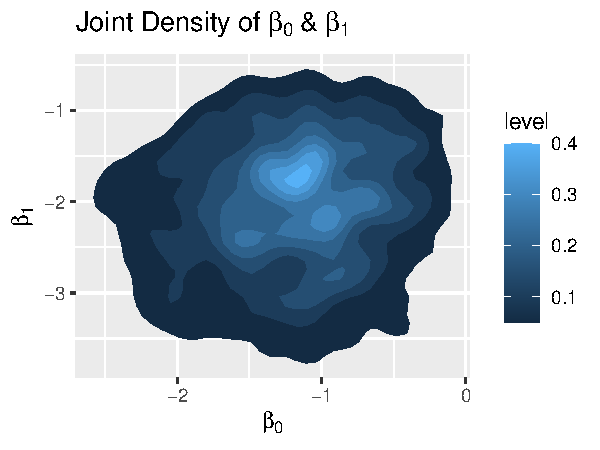
\includegraphics[width=\maxwidth]{figure/unnamed-chunk-11-1} 
\begin{kframe}\begin{alltt}
\hlcom{# b0,b2}
\hlkwd{ggplot}\hlstd{(Post.Samp1,} \hlkwd{aes}\hlstd{(}\hlkwc{x} \hlstd{= b0,} \hlkwc{y} \hlstd{= b2,} \hlkwc{fill} \hlstd{= ..level..))} \hlopt{+}
  \hlkwd{stat_density_2d}\hlstd{(}\hlkwc{geom} \hlstd{=} \hlstr{"polygon"}\hlstd{)} \hlopt{+}
\hlkwd{labs}\hlstd{(}\hlkwc{title} \hlstd{=} \hlkwd{bquote}\hlstd{(}\hlstr{"Joint Density of"} \hlopt{~} \hlstd{beta[}\hlnum{0}\hlstd{]} \hlopt{~} \hlstr{"&"} \hlopt{~} \hlstd{beta[}\hlnum{2}\hlstd{]),}
\hlkwc{x} \hlstd{=} \hlkwd{bquote}\hlstd{(beta[}\hlnum{0}\hlstd{]),} \hlkwc{y} \hlstd{=} \hlkwd{bquote}\hlstd{(beta[}\hlnum{2}\hlstd{]))}
\end{alltt}
\end{kframe}
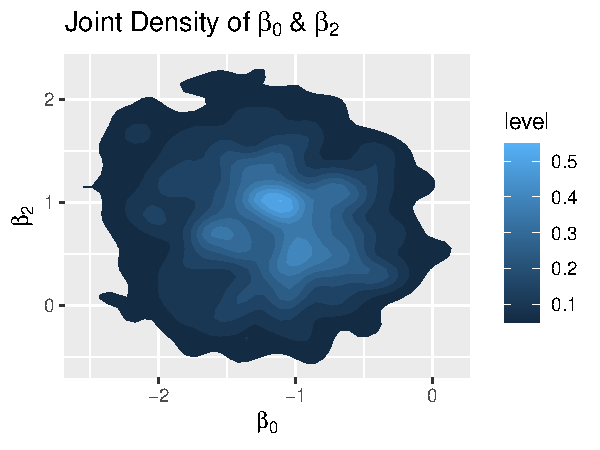
\includegraphics[width=\maxwidth]{figure/unnamed-chunk-11-2} 
\begin{kframe}\begin{alltt}
\hlcom{# b1,b2}
\hlkwd{ggplot}\hlstd{(Post.Samp1,} \hlkwd{aes}\hlstd{(}\hlkwc{x} \hlstd{= b1,} \hlkwc{y} \hlstd{= b2,} \hlkwc{fill} \hlstd{= ..level..))} \hlopt{+}
  \hlkwd{stat_density_2d}\hlstd{(}\hlkwc{geom} \hlstd{=} \hlstr{"polygon"}\hlstd{)} \hlopt{+}
\hlkwd{labs}\hlstd{(}\hlkwc{title} \hlstd{=} \hlkwd{bquote}\hlstd{(}\hlstr{"Joint Density of"} \hlopt{~} \hlstd{beta[}\hlnum{1}\hlstd{]} \hlopt{~} \hlstr{"&"} \hlopt{~} \hlstd{beta[}\hlnum{2}\hlstd{]),}
\hlkwc{x} \hlstd{=} \hlkwd{bquote}\hlstd{(beta[}\hlnum{1}\hlstd{]),} \hlkwc{y} \hlstd{=} \hlkwd{bquote}\hlstd{(beta[}\hlnum{2}\hlstd{]))}
\end{alltt}
\end{kframe}
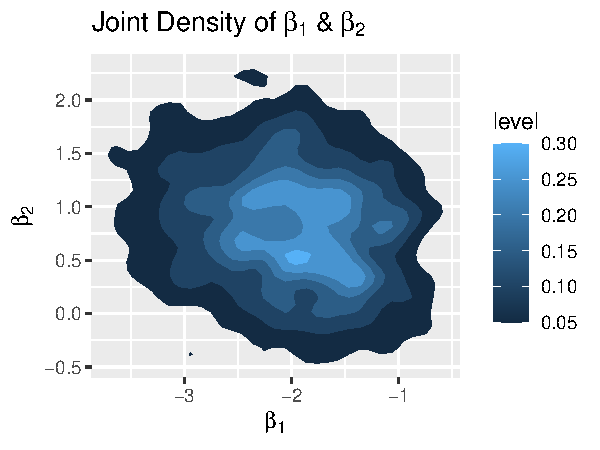
\includegraphics[width=\maxwidth]{figure/unnamed-chunk-11-3} 
\end{knitrout}
\par\end{center}

The most important thing to visualize is how we can model the posterior
probability distribution of that $\pi\left(y|\boldsymbol{X}\right)=P\left(Y=1|\boldsymbol{X}\right)=\frac{e^{\beta_{0}+\beta_{1}x_{1}+\beta_{2}x_{2}}}{1+e^{\beta_{0}+\beta_{1}x_{1}+\beta_{2}x_{2}}}$.
We use the sampled posterior values of $\boldsymbol{\beta}$ to plot
the approximate distribution of $\pi\left(y|\boldsymbol{X}\right)$
for some fixed value of $x_{1},x_{2}$. To see how the failure probability
depends on $x_{1}$ and $x_{2}$ we take different values and then
plot them. 
\begin{center}
\begin{knitrout}
\definecolor{shadecolor}{rgb}{0.969, 0.969, 0.969}\color{fgcolor}\begin{kframe}
\begin{alltt}
\hlstd{Post.Prob1} \hlkwb{<-} \hlkwa{function}\hlstd{(}\hlkwc{x.point}\hlstd{)}
\hlstd{\{}
  \hlstd{x.norm} \hlkwb{=} \hlkwa{NULL}
  \hlstd{x.norm[}\hlnum{1}\hlstd{]} \hlkwb{=} \hlstd{(x.point[}\hlnum{1}\hlstd{]} \hlopt{-} \hlkwd{mean}\hlstd{(Challeng}\hlopt{$}\hlstd{temp))}\hlopt{/}\hlkwd{sd}\hlstd{(Challeng}\hlopt{$}\hlstd{temp)}
  \hlstd{x.norm[}\hlnum{2}\hlstd{]} \hlkwb{=} \hlstd{(x.point[}\hlnum{2}\hlstd{]} \hlopt{-} \hlkwd{mean}\hlstd{(Challeng}\hlopt{$}\hlstd{pres))}\hlopt{/}\hlkwd{sd}\hlstd{(Challeng}\hlopt{$}\hlstd{pres)}
  \hlstd{x_val} \hlkwb{=} \hlkwd{matrix}\hlstd{(}\hlkwd{c}\hlstd{(}\hlnum{1}\hlstd{,x.norm),}\hlkwc{nrow} \hlstd{=} \hlnum{1}\hlstd{)}
  \hlstd{y_reg} \hlkwb{=} \hlstd{x_val}\hlopt\hlkwd{t}\hlstd{(Post.Samp1)}
  \hlstd{y_reg} \hlkwb{=} \hlkwd{as.vector}\hlstd{(y_reg)}
  \hlstd{Pi.Posterior} \hlkwb{<-} \hlkwd{exp}\hlstd{(y_reg)}\hlopt{/}\hlstd{(}\hlnum{1}\hlopt{+}\hlkwd{exp}\hlstd{(y_reg))}
  \hlkwd{return}\hlstd{(}\hlkwd{list}\hlstd{(}\hlstr{"samples"} \hlstd{= Pi.Posterior,}\hlstr{"post.mean"} \hlstd{=} \hlkwd{mean}\hlstd{(Pi.Posterior)))}
\hlstd{\}}

\hlcom{## Different choices of Tempareture and Pressure}
\hlstd{x.point1} \hlkwb{=} \hlkwd{c}\hlstd{(}\hlnum{75}\hlstd{,}\hlnum{5}\hlstd{)}
\hlstd{Samples.PRob} \hlkwb{<-} \hlkwd{Post.Prob1}\hlstd{(}\hlkwc{x.point} \hlstd{= x.point1)}\hlopt{$}\hlstd{samples}
\hlstd{Samples.PRob} \hlkwb{<-} \hlkwd{as.data.frame}\hlstd{(Samples.PRob)}
\hlkwd{ggplot}\hlstd{(}\hlkwc{data} \hlstd{= Samples.PRob,}\hlkwd{aes}\hlstd{(Samples.PRob))} \hlopt{+}
  \hlkwd{geom_density}\hlstd{(}\hlkwc{fill}\hlstd{=}\hlstr{"#69b3a2"}\hlstd{,} \hlkwc{color}\hlstd{=}\hlstr{"#e9ecef"}\hlstd{,} \hlkwc{alpha}\hlstd{=}\hlnum{0.8}\hlstd{)} \hlopt{+}
\hlkwd{labs}\hlstd{(}\hlkwc{title} \hlstd{=} \hlkwd{bquote}\hlstd{(}\hlstr{"Posterior Density Plot of"} \hlopt{~} \hlkwd{pi}\hlstd{(X)),}
\hlkwc{x} \hlstd{=} \hlkwd{bquote}\hlstd{(}\hlstr{"Temp = "} \hlopt{~} \hlkwd{.}\hlstd{(x.point1[}\hlnum{1}\hlstd{])} \hlopt{~} \hlstr{",Pres = "} \hlopt{~} \hlkwd{.}\hlstd{(x.point1[}\hlnum{2}\hlstd{])))}
\end{alltt}
\end{kframe}
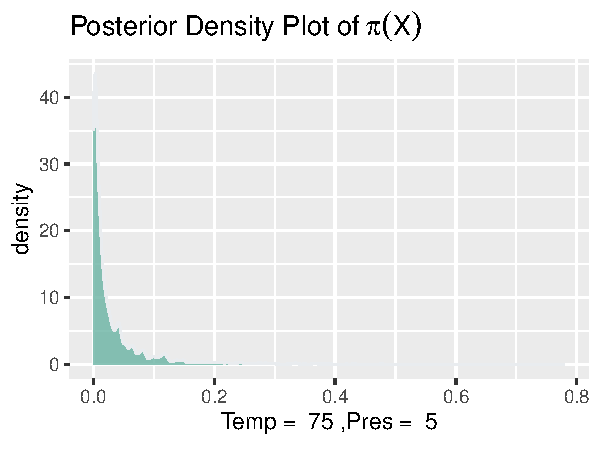
\includegraphics[width=\maxwidth]{figure/unnamed-chunk-12-1} 
\end{knitrout}
\par\end{center}

\begin{center}
\begin{knitrout}
\definecolor{shadecolor}{rgb}{0.969, 0.969, 0.969}\color{fgcolor}\begin{kframe}
\begin{alltt}
\hlstd{x.point1} \hlkwb{=} \hlkwd{c}\hlstd{(}\hlnum{75}\hlstd{,}\hlnum{100}\hlstd{)}
\hlstd{Samples.PRob} \hlkwb{<-} \hlkwd{Post.Prob1}\hlstd{(}\hlkwc{x.point} \hlstd{= x.point1)}\hlopt{$}\hlstd{samples}
\hlstd{Samples.PRob} \hlkwb{<-} \hlkwd{as.data.frame}\hlstd{(Samples.PRob)}
\hlkwd{ggplot}\hlstd{(}\hlkwc{data} \hlstd{= Samples.PRob,}\hlkwd{aes}\hlstd{(Samples.PRob))} \hlopt{+}
  \hlkwd{geom_density}\hlstd{(}\hlkwc{fill}\hlstd{=}\hlstr{"#69b3a2"}\hlstd{,} \hlkwc{color}\hlstd{=}\hlstr{"#e9ecef"}\hlstd{,} \hlkwc{alpha}\hlstd{=}\hlnum{0.8}\hlstd{)} \hlopt{+}
\hlkwd{labs}\hlstd{(}\hlkwc{title} \hlstd{=} \hlkwd{bquote}\hlstd{(}\hlstr{"Posterior Density Plot of"} \hlopt{~} \hlkwd{pi}\hlstd{(X)),}
\hlkwc{x} \hlstd{=} \hlkwd{bquote}\hlstd{(}\hlstr{"Temp = "} \hlopt{~} \hlkwd{.}\hlstd{(x.point1[}\hlnum{1}\hlstd{])} \hlopt{~} \hlstr{",Pres = "} \hlopt{~} \hlkwd{.}\hlstd{(x.point1[}\hlnum{2}\hlstd{])))}
\end{alltt}
\end{kframe}
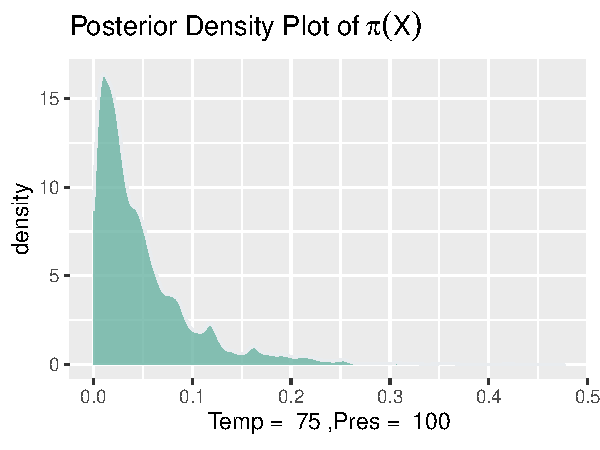
\includegraphics[width=\maxwidth]{figure/unnamed-chunk-13-1} 
\end{knitrout}
\par\end{center}

\begin{center}
\begin{knitrout}
\definecolor{shadecolor}{rgb}{0.969, 0.969, 0.969}\color{fgcolor}\begin{kframe}
\begin{alltt}
\hlstd{x.point1} \hlkwb{=} \hlkwd{c}\hlstd{(}\hlnum{50}\hlstd{,}\hlnum{30}\hlstd{)}
\hlstd{Samples.PRob} \hlkwb{<-} \hlkwd{Post.Prob1}\hlstd{(}\hlkwc{x.point} \hlstd{= x.point1)}\hlopt{$}\hlstd{samples}
\hlstd{Samples.PRob} \hlkwb{<-} \hlkwd{as.data.frame}\hlstd{(Samples.PRob)}
\hlkwd{ggplot}\hlstd{(}\hlkwc{data} \hlstd{= Samples.PRob,}\hlkwd{aes}\hlstd{(Samples.PRob))} \hlopt{+}
  \hlkwd{geom_density}\hlstd{(}\hlkwc{fill}\hlstd{=}\hlstr{"#69b3a2"}\hlstd{,} \hlkwc{color}\hlstd{=}\hlstr{"#e9ecef"}\hlstd{,} \hlkwc{alpha}\hlstd{=}\hlnum{0.8}\hlstd{)} \hlopt{+}
\hlkwd{labs}\hlstd{(}\hlkwc{title} \hlstd{=} \hlkwd{bquote}\hlstd{(}\hlstr{"Posterior Density Plot of"} \hlopt{~} \hlkwd{pi}\hlstd{(X)),}
\hlkwc{x} \hlstd{=} \hlkwd{bquote}\hlstd{(}\hlstr{"Temp = "} \hlopt{~} \hlkwd{.}\hlstd{(x.point1[}\hlnum{1}\hlstd{])} \hlopt{~} \hlstr{",Pres = "} \hlopt{~} \hlkwd{.}\hlstd{(x.point1[}\hlnum{2}\hlstd{])))}
\end{alltt}
\end{kframe}
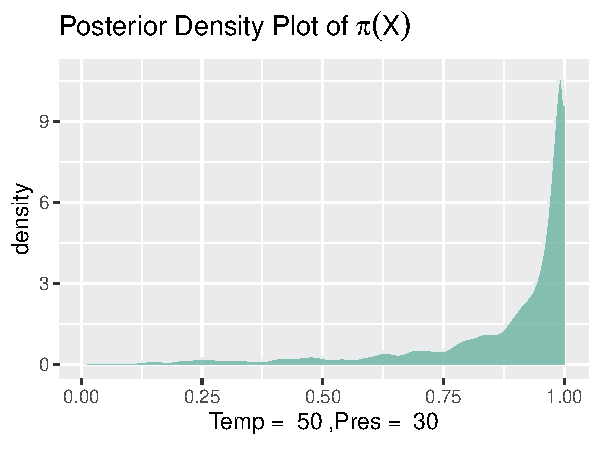
\includegraphics[width=\maxwidth]{figure/unnamed-chunk-14-1} 
\end{knitrout}
\par\end{center}

\begin{center}
\begin{knitrout}
\definecolor{shadecolor}{rgb}{0.969, 0.969, 0.969}\color{fgcolor}\begin{kframe}
\begin{alltt}
\hlstd{x.point1} \hlkwb{=} \hlkwd{c}\hlstd{(}\hlnum{50}\hlstd{,}\hlnum{100}\hlstd{)}
\hlstd{Samples.PRob} \hlkwb{<-} \hlkwd{Post.Prob1}\hlstd{(}\hlkwc{x.point} \hlstd{= x.point1)}\hlopt{$}\hlstd{samples}
\hlstd{Samples.PRob} \hlkwb{<-} \hlkwd{as.data.frame}\hlstd{(Samples.PRob)}
\hlkwd{ggplot}\hlstd{(}\hlkwc{data} \hlstd{= Samples.PRob,}\hlkwd{aes}\hlstd{(Samples.PRob))} \hlopt{+}
  \hlkwd{geom_density}\hlstd{(}\hlkwc{fill}\hlstd{=}\hlstr{"#69b3a2"}\hlstd{,} \hlkwc{color}\hlstd{=}\hlstr{"#e9ecef"}\hlstd{,} \hlkwc{alpha}\hlstd{=}\hlnum{0.8}\hlstd{)} \hlopt{+}
\hlkwd{labs}\hlstd{(}\hlkwc{title} \hlstd{=} \hlkwd{bquote}\hlstd{(}\hlstr{"Posterior Density Plot of"} \hlopt{~} \hlkwd{pi}\hlstd{(X)),}
\hlkwc{x} \hlstd{=} \hlkwd{bquote}\hlstd{(}\hlstr{"Temp = "} \hlopt{~} \hlkwd{.}\hlstd{(x.point1[}\hlnum{1}\hlstd{])} \hlopt{~} \hlstr{",Pres = "} \hlopt{~} \hlkwd{.}\hlstd{(x.point1[}\hlnum{2}\hlstd{])))}
\end{alltt}
\end{kframe}
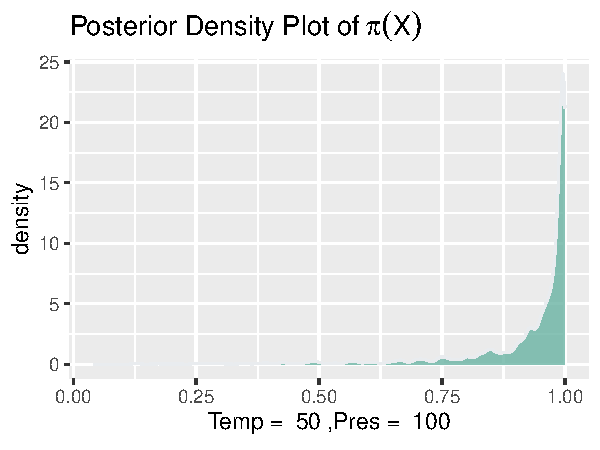
\includegraphics[width=\maxwidth]{figure/unnamed-chunk-15-1} 
\end{knitrout}
\par\end{center}

To see how the posterior mean of failure probability changes with
changing values of tempareture we calculate and several points and
then plot them joining by a line which gives :- (Here, we took fixed
value of pressure = 50 units)
\begin{center}
\begin{knitrout}
\definecolor{shadecolor}{rgb}{0.969, 0.969, 0.969}\color{fgcolor}\begin{kframe}
\begin{alltt}
\hlstd{temp.vals} \hlkwb{<-} \hlnum{40}\hlopt{:}\hlnum{100}
\hlstd{post.mean.vec} \hlkwb{<-} \hlkwd{sapply}\hlstd{(temp.vals,}
\hlkwa{function}\hlstd{(}\hlkwc{x}\hlstd{)\{}\hlkwd{return}\hlstd{(}\hlkwd{Post.Prob1}\hlstd{(}\hlkwc{x.point} \hlstd{=} \hlkwd{c}\hlstd{(x,}\hlnum{50}\hlstd{))}\hlopt{$}\hlstd{post.mean)\})}
\hlstd{post.mean} \hlkwb{<-} \hlkwd{data.frame}\hlstd{(}\hlstr{"x"} \hlstd{= temp.vals,}\hlstr{"post.mean"} \hlstd{= post.mean.vec)}
\hlstd{sd} \hlkwb{<-} \hlkwd{sapply}\hlstd{(temp.vals,}
\hlkwa{function}\hlstd{(}\hlkwc{x}\hlstd{)\{}\hlkwd{return}\hlstd{(}\hlkwd{sd}\hlstd{(}\hlkwd{Post.Prob1}\hlstd{(}\hlkwc{x.point} \hlstd{=} \hlkwd{c}\hlstd{(x,}\hlnum{50}\hlstd{))}\hlopt{$}\hlstd{samples))\})}
\hlkwd{ggplot}\hlstd{(post.mean)} \hlopt{+}
  \hlkwd{geom_line}\hlstd{(}\hlkwd{aes}\hlstd{(}\hlkwc{x} \hlstd{= temp.vals,}\hlkwc{y} \hlstd{= post.mean.vec))} \hlopt{+}
  \hlkwd{ylim}\hlstd{(}\hlkwd{c}\hlstd{(}\hlnum{0}\hlstd{,}\hlnum{1}\hlstd{))} \hlopt{+}
  \hlkwd{geom_point}\hlstd{(}\hlkwc{data} \hlstd{= Challeng,}\hlkwd{aes}\hlstd{(}\hlkwc{x} \hlstd{= temp,}\hlkwc{y} \hlstd{= Datas}\hlopt{$}\hlstd{Datas.fail))} \hlopt{+}
  \hlkwd{geom_errorbar}\hlstd{(}\hlkwd{aes}\hlstd{(}\hlkwc{x} \hlstd{= temp.vals,}\hlkwc{ymin} \hlstd{= post.mean.vec} \hlopt{-} \hlstd{sd}\hlopt{/}\hlnum{2}\hlstd{,}
  \hlkwc{ymax} \hlstd{= post.mean.vec} \hlopt{+} \hlstd{sd}\hlopt{/}\hlnum{2}\hlstd{),} \hlkwc{linewidth}\hlstd{=}\hlnum{0.4}\hlstd{,} \hlkwc{colour}\hlstd{=}\hlstr{"blue"}\hlstd{,} \hlkwc{alpha}\hlstd{=}\hlnum{0.9}
  \hlstd{,} \hlkwc{size}\hlstd{=}\hlnum{1.3}\hlstd{)} \hlopt{+}
  \hlkwd{labs}\hlstd{(}\hlkwc{title} \hlstd{=} \hlstr{"Posterior Mean of Failure Probability with Error Bars"}\hlstd{,}
  \hlkwc{x} \hlstd{=} \hlstr{"Tempareture"}\hlstd{,}\hlkwc{y} \hlstd{=} \hlstr{"Posterior Mean"}\hlstd{)}
\end{alltt}
\end{kframe}
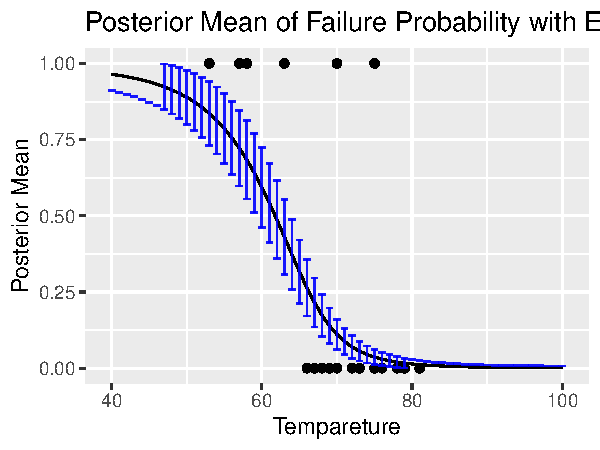
\includegraphics[width=\maxwidth]{figure/unnamed-chunk-16-1} 
\end{knitrout}
\par\end{center}
\author{\pagebreak}

\subsection*{Bayesian Logistic Model 2}

Since, we from the begining got enough evidence that Pressure is not
that signifcant a covariate hence, we thought of dropping this covariate
and then fitting a model assuming bivariate gaussian density. So our
model is :-
\[
P\left(Y_{i}=1|x_{i}\right)=\frac{e^{\beta_{0}+\beta_{1}x_{1i}}}{1+e^{\beta_{0}+\beta_{1}x_{1i}}}=\pi_{i},i=1,\dots,n
\]

The likelihood function of $\boldsymbol{\beta}$ given the observed
data $\boldsymbol{y,X}$ can be written as :-
\begin{align*}
f\left(\boldsymbol{y}|\boldsymbol{\beta},\boldsymbol{X}\right) & =\prod_{i=1}^{n}f\left(y_{i}|\boldsymbol{\beta},x_{i}\right)\\
 & =\prod_{i=1}^{n}\pi_{i}^{y_{i}}\left(1-\pi_{i}\right)^{1-y_{i}}\\
 & =\prod_{i=1}^{n}\left[\frac{e^{\beta_{0}+\beta_{1}x_{1i}}}{1+e^{\beta_{0}+\beta_{1}x_{1i}}}\right]^{y_{i}}\left[\frac{1}{1+e^{\beta_{0}+\beta_{1}x_{1i}}}\right]^{1-y_{i}}
\end{align*}

where, $\boldsymbol{\beta}=\begin{pmatrix}\beta_{0}\\
\beta_{1}
\end{pmatrix}\sim N_{2}\left(\boldsymbol{0},\lambda^{-1}\boldsymbol{I}_{2}\right)$.

Hence, the posterior of $\boldsymbol{\beta}$ can be written as :-
\begin{align*}
\pi\left(\boldsymbol{\beta}|\boldsymbol{x},\boldsymbol{y}\right) & \propto\pi\left(\boldsymbol{\beta}\right)f\left(\boldsymbol{y}|\boldsymbol{\beta},\boldsymbol{x}\right)\\
 & \propto\exp\left(-\frac{\lambda}{2}\boldsymbol{\beta}^{T}\boldsymbol{\beta}\right)\prod_{i=1}^{n}\left[\frac{e^{\beta_{0}+\beta_{1}x_{1i}}}{1+e^{\beta_{0}+\beta_{1}x_{1i}}}\right]^{y_{i}}\left[\frac{1}{1+e^{\beta_{0}+\beta_{1}x_{1i}}}\right]^{1-y_{i}}\\
 & \propto\exp\left(-\frac{\lambda}{2}\boldsymbol{\beta}^{T}\boldsymbol{\beta}\right)\prod\limits _{i=1}^{n}\left[\frac{e^{y_{i}\boldsymbol{\beta}^{T}\boldsymbol{x_{i}}}}{1+e^{\boldsymbol{\beta}^{T}\boldsymbol{x_{i}}}}\right]\left(=\widetilde{p}\left(\boldsymbol{\beta}\right)\right)
\end{align*}

not much change will be required for drawing posterior samples from
this density using MCMC. We do the exact same algorithm with no $\beta_{2}$
in this case and then get the following outcomes. The posterior densities
we plot one by one.

\begin{knitrout}
\definecolor{shadecolor}{rgb}{0.969, 0.969, 0.969}\color{fgcolor}\begin{kframe}
\begin{alltt}
\hlstd{likelihood2} \hlkwb{<-} \hlkwa{function}\hlstd{(}\hlkwc{X}\hlstd{,}\hlkwc{y}\hlstd{,}\hlkwc{beta}\hlstd{,}\hlkwc{lambda} \hlstd{=} \hlnum{0.01}\hlstd{,}\hlkwc{M} \hlstd{=} \hlnum{100}\hlstd{)}
\hlstd{\{}
  \hlstd{beta} \hlkwb{=} \hlkwd{matrix}\hlstd{(beta,}\hlkwc{nrow} \hlstd{=} \hlnum{1}\hlstd{)}
  \hlstd{a} \hlkwb{=} \hlkwd{exp}\hlstd{(}\hlopt{-}\hlstd{(lambda}\hlopt{/}\hlnum{2}\hlstd{)}\hlopt{*}\hlstd{beta}\hlopt\hlkwd{t}\hlstd{(beta))}
  \hlstd{b} \hlkwb{=} \hlkwd{exp}\hlstd{(y}\hlopt{*}\hlstd{(beta}\hlopt\hlkwd{t}\hlstd{(X)))}
  \hlstd{c} \hlkwb{=} \hlkwd{exp}\hlstd{(beta}\hlopt\hlkwd{t}\hlstd{(X))}
  \hlkwd{return}\hlstd{(M}\hlopt{*}\hlstd{a}\hlopt{*}\hlkwd{prod}\hlstd{(b}\hlopt{/}\hlstd{(}\hlnum{1}\hlopt{+}\hlstd{c)))}
\hlstd{\}}

\hlstd{MCMC.Sampler2} \hlkwb{<-} \hlkwa{function}\hlstd{(}\hlkwc{X}\hlstd{,}\hlkwc{y}\hlstd{,}\hlkwc{beta0}\hlstd{,}\hlkwc{B}\hlstd{,}\hlkwc{sg} \hlstd{=} \hlkwd{c}\hlstd{(}\hlnum{1}\hlstd{,}\hlnum{1}\hlstd{),}\hlkwc{showprogress} \hlstd{=} \hlnum{TRUE}\hlstd{,}\hlkwc{...}\hlstd{)}
\hlstd{\{}
  \hlstd{X} \hlkwb{=} \hlkwd{cbind}\hlstd{(}\hlkwd{rep}\hlstd{(}\hlnum{1}\hlstd{,}\hlkwd{nrow}\hlstd{(X)),X[,}\hlnum{1}\hlstd{])}
  \hlstd{beta0} \hlkwb{=} \hlkwd{matrix}\hlstd{(beta0,}\hlkwc{nrow} \hlstd{=} \hlnum{1}\hlstd{)}
  \hlstd{post.sample} \hlkwb{=} \hlkwd{c}\hlstd{(}\hlnum{0}\hlstd{,}\hlnum{0}\hlstd{)}
  \hlstd{beta1} \hlkwb{=} \hlstd{beta0}
  \hlstd{beta2} \hlkwb{=} \hlkwd{matrix}\hlstd{(}\hlkwd{c}\hlstd{(}\hlnum{0}\hlstd{,}\hlnum{0}\hlstd{),}\hlkwc{nrow} \hlstd{=} \hlnum{1}\hlstd{)}
  \hlstd{prog} \hlkwb{=} \hlkwd{txtProgressBar}\hlstd{(}\hlkwc{max} \hlstd{= B,}\hlkwc{style} \hlstd{=} \hlnum{3}\hlstd{)}
  \hlkwa{for}\hlstd{(i} \hlkwa{in} \hlnum{1}\hlopt{:}\hlstd{B)}
  \hlstd{\{}
    \hlstd{beta2[}\hlnum{1}\hlstd{]} \hlkwb{=} \hlstd{beta1[}\hlnum{1}\hlstd{]} \hlopt{+} \hlkwd{rnorm}\hlstd{(}\hlnum{1}\hlstd{,}\hlnum{0}\hlstd{,sg[}\hlnum{1}\hlstd{])}
    \hlstd{beta2[}\hlnum{2}\hlstd{]} \hlkwb{=} \hlstd{beta1[}\hlnum{2}\hlstd{]} \hlopt{+} \hlkwd{rnorm}\hlstd{(}\hlnum{1}\hlstd{,}\hlnum{0}\hlstd{,sg[}\hlnum{2}\hlstd{])}
    \hlstd{ratio} \hlkwb{=} \hlkwd{likelihood2}\hlstd{(X,y,}\hlkwc{beta} \hlstd{= beta2,...)}\hlopt{/}\hlkwd{likelihood2}\hlstd{(X,y,beta1,...)}
    \hlstd{unif} \hlkwb{=} \hlkwd{runif}\hlstd{(}\hlnum{1}\hlstd{)}
    \hlkwa{if}\hlstd{(unif} \hlopt{<=} \hlkwd{min}\hlstd{(}\hlnum{1}\hlstd{,ratio)) beta1}\hlkwb{=}\hlstd{beta2}
    \hlstd{post.sample} \hlkwb{=} \hlkwd{rbind}\hlstd{(post.sample,beta1)}
    \hlkwa{if}\hlstd{(showprogress)} \hlkwd{setTxtProgressBar}\hlstd{(}\hlkwc{pb} \hlstd{= prog,}\hlkwc{value} \hlstd{= i)}
    \hlstd{\}}
  \hlkwd{close}\hlstd{(prog)}
  \hlkwd{return}\hlstd{(post.sample)}
\hlstd{\}}
\end{alltt}
\end{kframe}
\end{knitrout}

Similarly, we draw samples from this posterior distribution and make
similar plots.

\begin{knitrout}
\definecolor{shadecolor}{rgb}{0.969, 0.969, 0.969}\color{fgcolor}\begin{kframe}
\begin{alltt}
\hlcom{# MCMC parameters}
\hlstd{B} \hlkwb{=} \hlnum{10}\hlopt{^}\hlnum{5}
\hlstd{n.thin} \hlkwb{=} \hlnum{5}

\hlcom{# Running the MCMC sampler}
\hlstd{Post.Sample2} \hlkwb{=} \hlkwd{MCMC.Sampler2}\hlstd{(}\hlkwc{X} \hlstd{= Datas[,}\hlnum{1}\hlopt{:}\hlnum{2}\hlstd{],}\hlkwc{y} \hlstd{= Datas}\hlopt{$}\hlstd{Datas.fail,}
\hlkwc{beta0} \hlstd{=} \hlkwd{c}\hlstd{(mod.glm}\hlopt{$}\hlstd{coefficients[}\hlnum{1}\hlstd{],mod.glm}\hlopt{$}\hlstd{coefficients[}\hlnum{2}\hlstd{]),B,}\hlkwc{sg} \hlstd{=} \hlkwd{c}\hlstd{(}\hlnum{3}\hlstd{,}\hlnum{3}\hlstd{),}\hlkwc{showprogress} \hlstd{=} \hlnum{FALSE}\hlstd{)}
\end{alltt}
\begin{verbatim}

  |                                                                            
  |                                                                      |   0%
\end{verbatim}
\begin{alltt}
\hlstd{Post.Sample2} \hlkwb{=} \hlstd{(Post.Sample2)[}\hlopt{-}\hlstd{(}\hlnum{1}\hlopt{:}\hlstd{(B}\hlopt{/}\hlnum{10}\hlstd{)),]}
\hlstd{n.length} \hlkwb{=} \hlkwd{nrow}\hlstd{(Post.Sample2)}
\hlstd{batch.size} \hlkwb{=} \hlkwd{floor}\hlstd{(n.length}\hlopt{/}\hlstd{n.thin)}
\hlstd{Post.Sample2} \hlkwb{=} \hlstd{Post.Sample2[n.thin}\hlopt{*}\hlstd{(}\hlnum{1}\hlopt{:}\hlstd{batch.size),]}
\hlstd{Post.Samp2} \hlkwb{=} \hlkwd{data.frame}\hlstd{(Post.Sample2)}
\hlkwd{names}\hlstd{(Post.Samp2)} \hlkwb{<-} \hlkwd{c}\hlstd{(}\hlstr{'b0'}\hlstd{,}\hlstr{'b1'}\hlstd{)}
\end{alltt}
\end{kframe}
\end{knitrout}

Now, using the generated posterior samples, we plot the posterior
densities of $\boldsymbol{\beta}$ individually. 
\begin{center}
\begin{knitrout}
\definecolor{shadecolor}{rgb}{0.969, 0.969, 0.969}\color{fgcolor}\begin{kframe}
\begin{alltt}
\hlcom{# Posterior distributions of beta0,beta1}
\hlkwd{ggplot}\hlstd{(}\hlkwc{data} \hlstd{= Post.Samp2,}\hlkwd{aes}\hlstd{(}\hlkwc{x}\hlstd{=b0))} \hlopt{+}
  \hlkwd{geom_density}\hlstd{(}\hlkwc{fill}\hlstd{=}\hlstr{"#69b3a2"}\hlstd{,} \hlkwc{color}\hlstd{=}\hlstr{"#e9ecef"}\hlstd{,} \hlkwc{alpha}\hlstd{=}\hlnum{0.8}\hlstd{)} \hlopt{+}
    \hlkwd{labs}\hlstd{(}\hlkwc{title} \hlstd{=} \hlkwd{bquote}\hlstd{(}\hlstr{"Density Plot of"} \hlopt{~} \hlstd{beta[}\hlnum{0}\hlstd{]),}\hlkwc{x} \hlstd{=} \hlkwd{bquote}\hlstd{(beta[}\hlnum{0}\hlstd{]))}
\end{alltt}
\end{kframe}
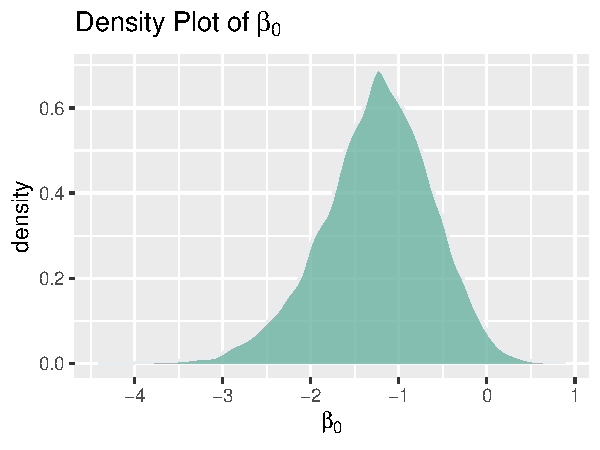
\includegraphics[width=\maxwidth]{figure/unnamed-chunk-19-1} 
\begin{kframe}\begin{alltt}
\hlkwd{ggplot}\hlstd{(}\hlkwc{data} \hlstd{= Post.Samp2,}\hlkwd{aes}\hlstd{(}\hlkwc{x}\hlstd{=b1))} \hlopt{+}
  \hlkwd{geom_density}\hlstd{(}\hlkwc{fill}\hlstd{=}\hlstr{"#69b3a2"}\hlstd{,} \hlkwc{color}\hlstd{=}\hlstr{"#e9ecef"}\hlstd{,} \hlkwc{alpha}\hlstd{=}\hlnum{0.8}\hlstd{)} \hlopt{+}
  \hlkwd{labs}\hlstd{(}\hlkwc{title} \hlstd{=} \hlkwd{bquote}\hlstd{(}\hlstr{"Density Plot of"} \hlopt{~} \hlstd{beta[}\hlnum{1}\hlstd{]),}\hlkwc{x} \hlstd{=} \hlkwd{bquote}\hlstd{(beta[}\hlnum{1}\hlstd{]))}
\end{alltt}
\end{kframe}
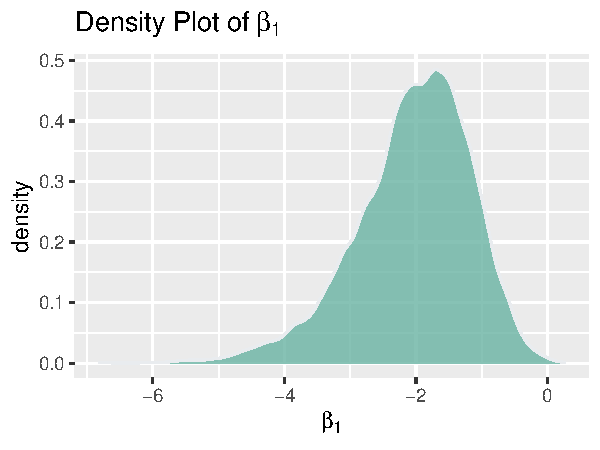
\includegraphics[width=\maxwidth]{figure/unnamed-chunk-19-2} 
\end{knitrout}
\par\end{center}

The posterior means for the three parameters are :-

\begin{knitrout}
\definecolor{shadecolor}{rgb}{0.969, 0.969, 0.969}\color{fgcolor}\begin{kframe}
\begin{alltt}
\hlstd{m1} \hlkwb{=} \hlkwd{apply}\hlstd{(Post.Samp1,} \hlnum{2}\hlstd{, mean)}
\hlstd{m2} \hlkwb{=} \hlstd{mod.glm}\hlopt{$}\hlstd{coefficients}
\hlkwd{data.frame}\hlstd{(}\hlstr{"Posterior.Means"} \hlstd{= m1,}\hlstr{"Logistic.Coef"} \hlstd{= m2)}
\end{alltt}
\begin{verbatim}
   Posterior.Means Logistic.Coef
b0      -1.2623902    -1.0543469
b1      -2.2007295    -1.7045661
b2       0.8659067     0.6728236
\end{verbatim}
\end{kframe}
\end{knitrout}

To know whether these estimates are more or less consistent or not
(ergodicity) we plot the cumulative means of these posterior samples.
\begin{center}
\begin{knitrout}
\definecolor{shadecolor}{rgb}{0.969, 0.969, 0.969}\color{fgcolor}\begin{kframe}
\begin{alltt}
\hlcom{# plotting the mean cumulatively w.r.t sample size}
\hlstd{b0.mean.cum} \hlkwb{<-} \hlkwd{cumsum}\hlstd{(Post.Samp2}\hlopt{$}\hlstd{b0)}\hlopt{/}\hlstd{(}\hlnum{1}\hlopt{:}\hlkwd{nrow}\hlstd{(Post.Samp2))}
\hlstd{b1.mean.cum} \hlkwb{<-} \hlkwd{cumsum}\hlstd{(Post.Samp2}\hlopt{$}\hlstd{b1)}\hlopt{/}\hlstd{(}\hlnum{1}\hlopt{:}\hlkwd{nrow}\hlstd{(Post.Samp2))}
\hlcom{# plot of means with increasing sample size}
\hlkwd{plot}\hlstd{(b0.mean.cum,}\hlkwc{type} \hlstd{=} \hlstr{"l"}\hlstd{,}
\hlkwc{main} \hlstd{=} \hlkwd{bquote}\hlstd{(}\hlstr{"posterior mean of "} \hlopt{~} \hlstd{beta[}\hlnum{0}\hlstd{]),}\hlkwc{xlab} \hlstd{=} \hlkwd{bquote}\hlstd{(beta[}\hlnum{0}\hlstd{]),}\hlkwc{ylab} \hlstd{=} \hlstr{"mean"}\hlstd{)}
\end{alltt}
\end{kframe}
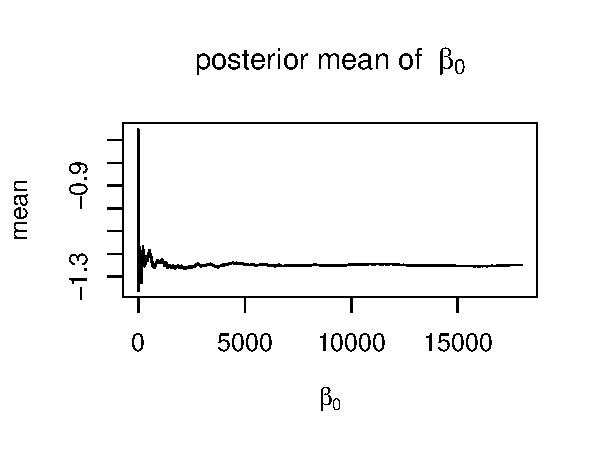
\includegraphics[width=\maxwidth]{figure/unnamed-chunk-21-1} 
\begin{kframe}\begin{alltt}
\hlkwd{plot}\hlstd{(b1.mean.cum,}\hlkwc{type} \hlstd{=} \hlstr{"l"}\hlstd{,}
\hlkwc{main} \hlstd{=} \hlkwd{bquote}\hlstd{(}\hlstr{"posterior mean of "} \hlopt{~} \hlstd{beta[}\hlnum{1}\hlstd{]),}\hlkwc{xlab} \hlstd{=} \hlkwd{bquote}\hlstd{(beta[}\hlnum{1}\hlstd{]),}\hlkwc{ylab} \hlstd{=} \hlstr{"mean"}\hlstd{)}
\end{alltt}
\end{kframe}
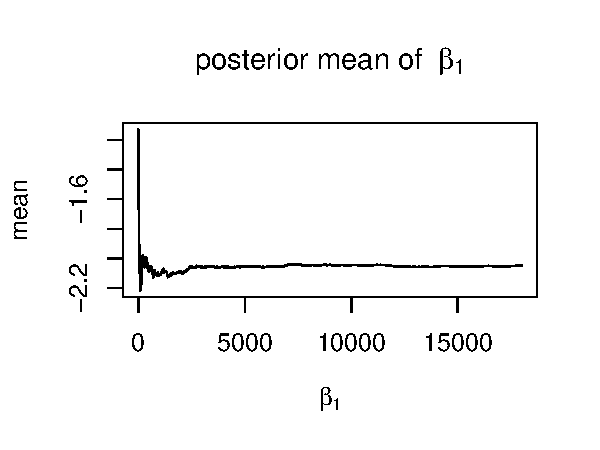
\includegraphics[width=\maxwidth]{figure/unnamed-chunk-21-2} 
\end{knitrout}
\par\end{center}

With increasing sample size, we can see that the mean more or less
gets stabilized indicating their consistency.

Here's another plot which may provide better idea through bivariate
density plots taking two variables at a time where the density is
shown using varying colour density.
\begin{center}
\begin{knitrout}
\definecolor{shadecolor}{rgb}{0.969, 0.969, 0.969}\color{fgcolor}\begin{kframe}
\begin{alltt}
\hlcom{# b0,b1}
\hlkwd{ggplot}\hlstd{(Post.Samp2,} \hlkwd{aes}\hlstd{(}\hlkwc{x} \hlstd{= b0,} \hlkwc{y} \hlstd{= b1,} \hlkwc{fill} \hlstd{= ..level..))} \hlopt{+}
  \hlkwd{stat_density_2d}\hlstd{(}\hlkwc{geom} \hlstd{=} \hlstr{"polygon"}\hlstd{)} \hlopt{+}
\hlkwd{labs}\hlstd{(}\hlkwc{title} \hlstd{=} \hlkwd{bquote}\hlstd{(}\hlstr{"Joint Density of"} \hlopt{~} \hlstd{beta[}\hlnum{0}\hlstd{]} \hlopt{~} \hlstr{"&"} \hlopt{~} \hlstd{beta[}\hlnum{1}\hlstd{]),}
\hlkwc{x} \hlstd{=} \hlkwd{bquote}\hlstd{(beta[}\hlnum{0}\hlstd{]),} \hlkwc{y} \hlstd{=} \hlkwd{bquote}\hlstd{(beta[}\hlnum{1}\hlstd{]))}
\end{alltt}
\end{kframe}
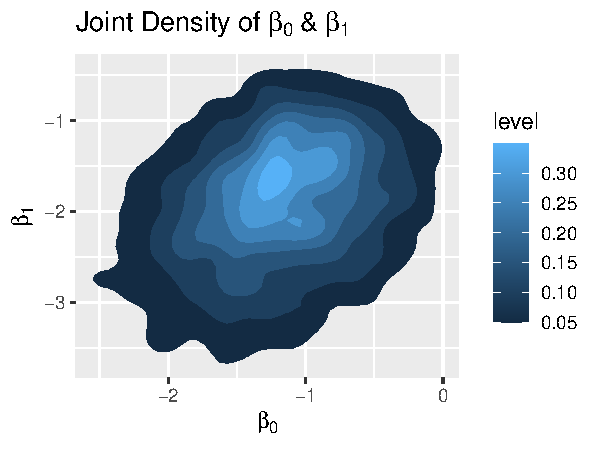
\includegraphics[width=\maxwidth]{figure/unnamed-chunk-22-1} 
\end{knitrout}
\par\end{center}

The most important thing to visualize is how we can model the posterior
probability distribution of that $\pi\left(y|\boldsymbol{X}\right)=P\left(Y=1|\boldsymbol{X}\right)=\frac{e^{\beta_{0}+\beta_{1}x_{1}}}{1+e^{\beta_{0}+\beta_{1}x_{1}}}$.
We use the sampled posterior values of $\boldsymbol{\beta}$ to plot
the approximate distribution of $\pi\left(y|\boldsymbol{X}\right)$
for some fixed value of $x_{1},x_{2}$. To see how the failure probability
depends on $x_{1}$ we take different values and then plot them.
\begin{center}
\begin{knitrout}
\definecolor{shadecolor}{rgb}{0.969, 0.969, 0.969}\color{fgcolor}\begin{kframe}
\begin{alltt}
\hlstd{Post.Prob2} \hlkwb{<-} \hlkwa{function}\hlstd{(}\hlkwc{x.point}\hlstd{)}
\hlstd{\{}
  \hlstd{x.norm} \hlkwb{=} \hlstd{(x.point[}\hlnum{1}\hlstd{]} \hlopt{-} \hlkwd{mean}\hlstd{(Challeng}\hlopt{$}\hlstd{temp))}\hlopt{/}\hlkwd{sd}\hlstd{(Challeng}\hlopt{$}\hlstd{temp)}
  \hlstd{x_val} \hlkwb{=} \hlkwd{matrix}\hlstd{(}\hlkwd{c}\hlstd{(}\hlnum{1}\hlstd{,x.norm),}\hlkwc{nrow} \hlstd{=} \hlnum{1}\hlstd{)}
  \hlstd{y_reg} \hlkwb{=} \hlstd{x_val}\hlopt\hlkwd{t}\hlstd{(Post.Samp2)}
  \hlstd{y_reg} \hlkwb{=} \hlkwd{as.vector}\hlstd{(y_reg)}
  \hlstd{Pi.Posterior} \hlkwb{<-} \hlkwd{exp}\hlstd{(y_reg)}\hlopt{/}\hlstd{(}\hlnum{1}\hlopt{+}\hlkwd{exp}\hlstd{(y_reg))}
  \hlkwd{return}\hlstd{(}\hlkwd{list}\hlstd{(}\hlstr{"samples"} \hlstd{= Pi.Posterior,}\hlstr{"post.mean"} \hlstd{=} \hlkwd{mean}\hlstd{(Pi.Posterior)))}
\hlstd{\}}

\hlcom{## Different choices of Tempareture and Pressure}
\hlstd{x.point1} \hlkwb{=} \hlnum{75}
\hlstd{Samples.PRob} \hlkwb{<-} \hlkwd{Post.Prob2}\hlstd{(}\hlkwc{x.point} \hlstd{= x.point1)}\hlopt{$}\hlstd{samples}
\hlstd{Samples.PRob} \hlkwb{<-} \hlkwd{as.data.frame}\hlstd{(Samples.PRob)}
\hlkwd{ggplot}\hlstd{(}\hlkwc{data} \hlstd{= Samples.PRob,}\hlkwd{aes}\hlstd{(Samples.PRob))} \hlopt{+}
  \hlkwd{geom_density}\hlstd{(}\hlkwc{fill}\hlstd{=}\hlstr{"#69b3a2"}\hlstd{,} \hlkwc{color}\hlstd{=}\hlstr{"#e9ecef"}\hlstd{,} \hlkwc{alpha}\hlstd{=}\hlnum{0.8}\hlstd{)} \hlopt{+}
  \hlkwd{labs}\hlstd{(}\hlkwc{title} \hlstd{=} \hlkwd{bquote}\hlstd{(}\hlstr{"Posterior Density Plot of"} \hlopt{~} \hlkwd{pi}\hlstd{(X)),}
\hlkwc{x} \hlstd{=} \hlkwd{bquote}\hlstd{(}\hlstr{"Temp = "} \hlopt{~} \hlkwd{.}\hlstd{(x.point1)))}
\end{alltt}
\end{kframe}
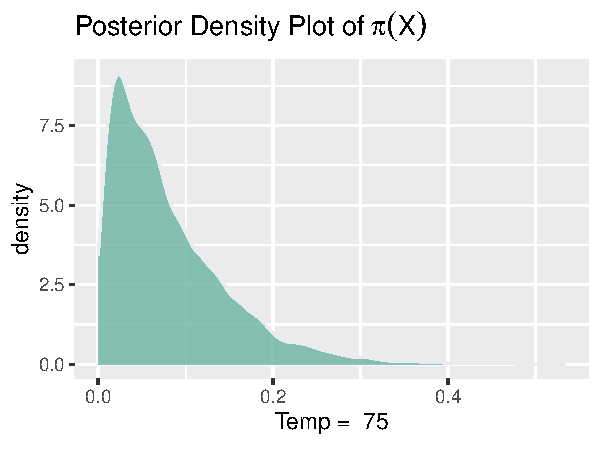
\includegraphics[width=\maxwidth]{figure/unnamed-chunk-23-1} 
\end{knitrout}
\par\end{center}

\begin{center}
\begin{knitrout}
\definecolor{shadecolor}{rgb}{0.969, 0.969, 0.969}\color{fgcolor}\begin{kframe}
\begin{alltt}
\hlstd{x.point1} \hlkwb{=} \hlnum{65}
\hlstd{Samples.PRob} \hlkwb{<-} \hlkwd{Post.Prob2}\hlstd{(}\hlkwc{x.point} \hlstd{= x.point1)}\hlopt{$}\hlstd{samples}
\hlstd{Samples.PRob} \hlkwb{<-} \hlkwd{as.data.frame}\hlstd{(Samples.PRob)}
\hlkwd{ggplot}\hlstd{(}\hlkwc{data} \hlstd{= Samples.PRob,}\hlkwd{aes}\hlstd{(Samples.PRob))} \hlopt{+}
  \hlkwd{geom_density}\hlstd{(}\hlkwc{fill}\hlstd{=}\hlstr{"#69b3a2"}\hlstd{,} \hlkwc{color}\hlstd{=}\hlstr{"#e9ecef"}\hlstd{,} \hlkwc{alpha}\hlstd{=}\hlnum{0.8}\hlstd{)} \hlopt{+}
  \hlkwd{labs}\hlstd{(}\hlkwc{title} \hlstd{=} \hlkwd{bquote}\hlstd{(}\hlstr{"Posterior Density Plot of"} \hlopt{~} \hlkwd{pi}\hlstd{(X)),}
\hlkwc{x} \hlstd{=} \hlkwd{bquote}\hlstd{(}\hlstr{"Temp = "} \hlopt{~} \hlkwd{.}\hlstd{(x.point1)))}
\end{alltt}
\end{kframe}
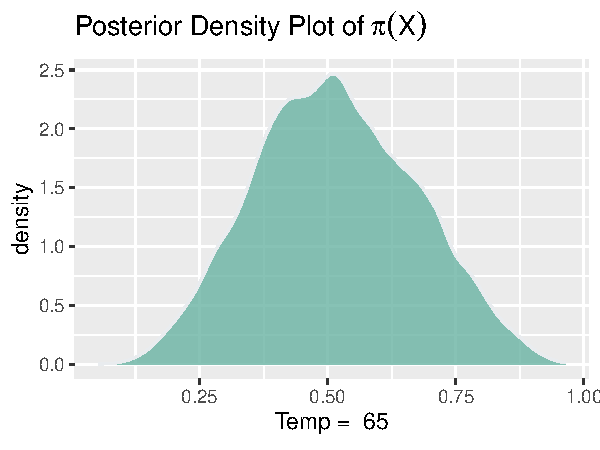
\includegraphics[width=\maxwidth]{figure/unnamed-chunk-24-1} 
\end{knitrout}
\par\end{center}

\begin{center}
\begin{knitrout}
\definecolor{shadecolor}{rgb}{0.969, 0.969, 0.969}\color{fgcolor}\begin{kframe}
\begin{alltt}
\hlstd{x.point1} \hlkwb{=} \hlnum{50}
\hlstd{Samples.PRob} \hlkwb{<-} \hlkwd{Post.Prob2}\hlstd{(}\hlkwc{x.point} \hlstd{= x.point1)}\hlopt{$}\hlstd{samples}
\hlstd{Samples.PRob} \hlkwb{<-} \hlkwd{as.data.frame}\hlstd{(Samples.PRob)}
\hlkwd{ggplot}\hlstd{(}\hlkwc{data} \hlstd{= Samples.PRob,}\hlkwd{aes}\hlstd{(Samples.PRob))} \hlopt{+}
  \hlkwd{geom_density}\hlstd{(}\hlkwc{fill}\hlstd{=}\hlstr{"#69b3a2"}\hlstd{,} \hlkwc{color}\hlstd{=}\hlstr{"#e9ecef"}\hlstd{,} \hlkwc{alpha}\hlstd{=}\hlnum{0.8}\hlstd{)} \hlopt{+}
  \hlkwd{labs}\hlstd{(}\hlkwc{title} \hlstd{=} \hlkwd{bquote}\hlstd{(}\hlstr{"Posterior Density Plot of"} \hlopt{~} \hlkwd{pi}\hlstd{(X)),}
\hlkwc{x} \hlstd{=} \hlkwd{bquote}\hlstd{(}\hlstr{"Temp = "} \hlopt{~} \hlkwd{.}\hlstd{(x.point1)))}
\end{alltt}
\end{kframe}
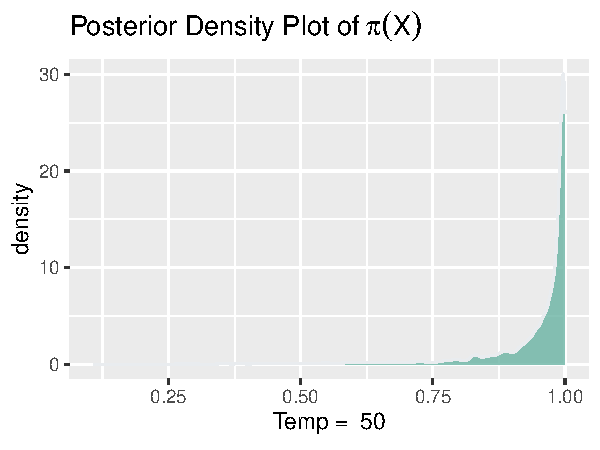
\includegraphics[width=\maxwidth]{figure/unnamed-chunk-25-1} 
\end{knitrout}
\par\end{center}

To see how the posterior mean of failure probability changes with
changing values of tempareture we calculate and several points and
then plot them joining by a line which gives :- (Here, we took fixed
value of pressure = 50 units)
\begin{center}
\begin{knitrout}
\definecolor{shadecolor}{rgb}{0.969, 0.969, 0.969}\color{fgcolor}\begin{kframe}
\begin{alltt}
\hlcom{# Plotting}
\hlstd{temp.vals} \hlkwb{<-} \hlnum{40}\hlopt{:}\hlnum{100}
\hlstd{post.mean.vec} \hlkwb{<-} \hlkwd{sapply}\hlstd{(temp.vals,} \hlkwa{function}\hlstd{(}\hlkwc{x}\hlstd{)\{}\hlkwd{return}\hlstd{(}\hlkwd{Post.Prob2}\hlstd{(}\hlkwc{x.point} \hlstd{= x)}\hlopt{$}\hlstd{post.mean)\})}
\hlstd{post.mean} \hlkwb{<-} \hlkwd{data.frame}\hlstd{(}\hlstr{"x"} \hlstd{= temp.vals,}\hlstr{"post.mean"} \hlstd{= post.mean.vec)}
\hlstd{sd} \hlkwb{<-} \hlkwd{sapply}\hlstd{(temp.vals,} \hlkwa{function}\hlstd{(}\hlkwc{x}\hlstd{)\{}\hlkwd{return}\hlstd{(}\hlkwd{sd}\hlstd{(}\hlkwd{Post.Prob2}\hlstd{(}\hlkwc{x.point} \hlstd{= x)}\hlopt{$}\hlstd{samples))\})}
\hlkwd{ggplot}\hlstd{(post.mean)} \hlopt{+}
  \hlkwd{geom_line}\hlstd{(}\hlkwd{aes}\hlstd{(}\hlkwc{x} \hlstd{= temp.vals,}\hlkwc{y} \hlstd{= post.mean.vec))} \hlopt{+}
  \hlkwd{ylim}\hlstd{(}\hlkwd{c}\hlstd{(}\hlnum{0}\hlstd{,}\hlnum{1}\hlstd{))} \hlopt{+}
  \hlkwd{geom_point}\hlstd{(}\hlkwc{data} \hlstd{= Challeng,}\hlkwd{aes}\hlstd{(}\hlkwc{x} \hlstd{= temp,}\hlkwc{y} \hlstd{= Datas}\hlopt{$}\hlstd{Datas.fail))} \hlopt{+}
  \hlkwd{geom_errorbar}\hlstd{(}\hlkwd{aes}\hlstd{(}\hlkwc{x} \hlstd{= temp.vals,}\hlkwc{ymin} \hlstd{= post.mean.vec} \hlopt{-} \hlstd{sd}\hlopt{/}\hlnum{2}\hlstd{,}
                    \hlkwc{ymax} \hlstd{= post.mean.vec} \hlopt{+} \hlstd{sd}\hlopt{/}\hlnum{2}\hlstd{),}
\hlkwc{linewidth}\hlstd{=}\hlnum{0.4}\hlstd{,} \hlkwc{colour}\hlstd{=}\hlstr{"blue"}\hlstd{,} \hlkwc{alpha}\hlstd{=}\hlnum{0.9}
                \hlstd{,} \hlkwc{size}\hlstd{=}\hlnum{1.3}\hlstd{)} \hlopt{+}
  \hlkwd{labs}\hlstd{(}\hlkwc{title} \hlstd{=} \hlstr{"Posterior Mean of Failure Probability with Error Bars"}\hlstd{,}
       \hlkwc{x} \hlstd{=} \hlstr{"Tempareture"}\hlstd{,}\hlkwc{y} \hlstd{=} \hlstr{"Posterior Mean"}\hlstd{)}
\end{alltt}
\end{kframe}
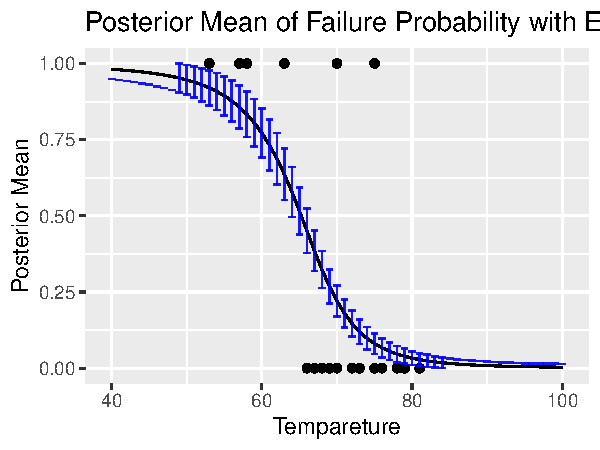
\includegraphics[width=\maxwidth]{figure/unnamed-chunk-26-1} 
\end{knitrout}
\par\end{center}
\author{\pagebreak}

\subsection*{Model Comparison}

So we have the two models :-
\begin{align*}
M_{0}: & X\text{ has density }f_{0}\left(\boldsymbol{y}|\boldsymbol{\beta,x}\right)\text{ where }\boldsymbol{\beta=\begin{pmatrix}\beta_{0},\beta_{1}\end{pmatrix}}\\
M_{1}: & X\text{ has density }f_{1}\left(\boldsymbol{y}|\boldsymbol{\beta,x}\right)\text{ where }\boldsymbol{\beta=\begin{pmatrix}\beta_{0},\beta_{1},\beta_{2}\end{pmatrix}}
\end{align*}
 We will use the Bayes Factor $B_{01}\left(\boldsymbol{X}\right)=\frac{m_{0}\left(\boldsymbol{X,y}\right)}{m_{1}\left(\boldsymbol{X,y}\right)}$
where 
\begin{align*}
m_{0}\left(\boldsymbol{X,y}\right) & =\int f_{0}\left(\boldsymbol{y}|\boldsymbol{\beta},\boldsymbol{x}\right)\pi_{0}\left(\boldsymbol{\beta}\right)d\boldsymbol{\beta}\\
 & =\int\prod\limits _{i=1}^{n}\left[\frac{e^{y_{i}\boldsymbol{\beta}^{T}\boldsymbol{x_{i}}}}{1+e^{\boldsymbol{\beta}^{T}\boldsymbol{x_{i}}}}\right]\pi_{0}\left(\boldsymbol{\beta}\right)d\boldsymbol{\beta}\\
 & \approx\frac{1}{N}\sum_{i=1}^{N}f_{0}\left(\boldsymbol{y}|\boldsymbol{\beta}^{\left(i\right)},\boldsymbol{x}\right)\text{ where }\\
 & \boldsymbol{\beta}^{\left(i\right)}|H_{0}\sim f_{0}\left(\boldsymbol{y}|\boldsymbol{\beta,x}\right)
\end{align*}

and similarly, compute $m_{1}\left(\boldsymbol{X,y}\right)$ and calculate
the approximate value of $BF_{10}$ as :-
\[
BF_{10}=\frac{m_{1}\left(\boldsymbol{X,y}\right)}{m_{0}\left(\boldsymbol{X,y}\right)}
\]

we use naive monte approximate the values and obtain the approximate
value of $\log_{10}\left(BF_{10}\right)$ as $\approx-2.065358$hence,
there is almost no evidence to reject $H_{0}$ so this again signifies
that the pressure variable is not signifcant. But if we rather consider
$\beta_{1}$ to be $0$ in null and not zero in alternate then we
obtain the value of $\log_{10}\left(BF_{10}\right)$ as$\approx2$
which signifies that there is a strong evidence to reject $H_{0}$
and hence tempareture must be an important variable.
\author{\pagebreak}

\section*{Bayesian Model 2}

As another ``different'' model we propose a similar model where,
we choose the ``probit'' link function instead of ``logit'' link.
Then we can write the probability of failure as :-
\[
P\left(Y_{i}=1|x_{i}\right)=\Phi\left(\beta_{0}+\beta_{1}x_{1i}\right)=\pi_{i},i=1,\dots,n
\]

as can be seen we don't keep pressure as a covariate here because
anyhow it won't have much significance evident from all the analysis
done before.

The likelihood function of $\boldsymbol{\beta}$ given the observed
data $\boldsymbol{y,X}$ can be written as :-
\begin{align*}
f\left(\boldsymbol{y}|\boldsymbol{\beta},\boldsymbol{X}\right) & =\prod_{i=1}^{n}f\left(y_{i}|\boldsymbol{\beta},x_{i}\right)\\
 & =\prod_{i=1}^{n}\pi_{i}^{y_{i}}\left(1-\pi_{i}\right)^{1-y_{i}}\\
 & =\prod_{i=1}^{n}\left\{ \Phi\left(\beta_{0}+\beta_{1}x_{1i}\right)\right\} ^{y_{i}}\left\{ 1-\Phi\left(\beta_{0}+\beta_{1}x_{1i}\right)\right\} ^{1-y_{i}}
\end{align*}

where, $\boldsymbol{\beta}=\begin{pmatrix}\beta_{0}\\
\beta_{1}
\end{pmatrix}\sim N_{2}\left(\boldsymbol{0},\lambda^{-1}\boldsymbol{I}_{2}\right)$.

Hence, the posterior of $\boldsymbol{\beta}$ can be written as :-
\begin{align*}
\pi\left(\boldsymbol{\beta}|\boldsymbol{x},\boldsymbol{y}\right) & \propto\pi\left(\boldsymbol{\beta}\right)f\left(\boldsymbol{y}|\boldsymbol{\beta},\boldsymbol{x}\right)\\
 & \propto\exp\left(-\frac{\lambda}{2}\boldsymbol{\beta}^{T}\boldsymbol{\beta}\right)\prod_{i=1}^{n}\left\{ \Phi\left(\beta_{0}+\beta_{1}x_{1i}\right)\right\} ^{y_{i}}\left\{ 1-\Phi\left(\beta_{0}+\beta_{1}x_{1i}\right)\right\} ^{1-y_{i}}\\
 & \propto\exp\left(-\frac{\lambda}{2}\boldsymbol{\beta}^{T}\boldsymbol{\beta}\right)\prod_{i=1}^{n}\left\{ \Phi\left(\beta_{0}+\beta_{1}x_{1i}\right)\right\} ^{y_{i}}\left\{ 1-\Phi\left(\beta_{0}+\beta_{1}x_{1i}\right)\right\} ^{1-y_{i}}\left(=\widetilde{p}\left(\boldsymbol{\beta}\right)\right)
\end{align*}

and here too we do similar analysis and plot the results one by one
:-

Here is the MCMC sampler (Using MH algorithm) that we have written
manually :-

\begin{knitrout}
\definecolor{shadecolor}{rgb}{0.969, 0.969, 0.969}\color{fgcolor}\begin{kframe}
\begin{alltt}
\hlstd{likelihood2.1} \hlkwb{<-} \hlkwa{function}\hlstd{(}\hlkwc{X}\hlstd{,}\hlkwc{y}\hlstd{,}\hlkwc{beta}\hlstd{,}\hlkwc{lambda} \hlstd{=} \hlnum{0.01}\hlstd{,}\hlkwc{M} \hlstd{=} \hlnum{100}\hlstd{)}
\hlstd{\{}
  \hlstd{beta} \hlkwb{=} \hlkwd{matrix}\hlstd{(beta,}\hlkwc{nrow} \hlstd{=} \hlnum{1}\hlstd{)}
  \hlstd{a} \hlkwb{=} \hlkwd{exp}\hlstd{(}\hlopt{-}\hlstd{(lambda}\hlopt{/}\hlnum{2}\hlstd{)}\hlopt{*}\hlstd{beta}\hlopt\hlkwd{t}\hlstd{(beta))}
  \hlstd{b} \hlkwb{=} \hlkwd{pnorm}\hlstd{(}\hlkwc{q} \hlstd{= beta}\hlopt\hlkwd{t}\hlstd{(X))}
  \hlstd{c} \hlkwb{=} \hlstd{(b}\hlopt{^}\hlstd{y)}\hlopt{*}\hlstd{((}\hlnum{1}\hlopt{-}\hlstd{b)}\hlopt{^}\hlstd{(}\hlnum{1}\hlopt{-}\hlstd{y))}
  \hlkwd{return}\hlstd{(M}\hlopt{*}\hlstd{a}\hlopt{*}\hlkwd{prod}\hlstd{(c))}
\hlstd{\}}

\hlstd{MCMC.Sampler2.1} \hlkwb{<-} \hlkwa{function}\hlstd{(}\hlkwc{X}\hlstd{,}\hlkwc{y}\hlstd{,}\hlkwc{beta0}\hlstd{,}\hlkwc{B}\hlstd{,}\hlkwc{sg} \hlstd{=} \hlkwd{c}\hlstd{(}\hlnum{1}\hlstd{,}\hlnum{1}\hlstd{),}
\hlkwc{showprogress} \hlstd{=} \hlnum{TRUE}\hlstd{,}\hlkwc{lambda} \hlstd{=} \hlnum{0.01}\hlstd{)}
\hlstd{\{}
  \hlstd{X} \hlkwb{=} \hlkwd{cbind}\hlstd{(}\hlkwd{rep}\hlstd{(}\hlnum{1}\hlstd{,}\hlkwd{nrow}\hlstd{(X)),X)}
  \hlstd{beta0} \hlkwb{=} \hlkwd{matrix}\hlstd{(beta0,}\hlkwc{nrow} \hlstd{=} \hlnum{1}\hlstd{)}
  \hlstd{post.sample} \hlkwb{=} \hlkwd{c}\hlstd{(}\hlnum{0}\hlstd{,}\hlnum{0}\hlstd{,}\hlnum{0}\hlstd{)}
  \hlstd{beta1} \hlkwb{=} \hlstd{beta0}
  \hlstd{beta2} \hlkwb{=} \hlkwd{matrix}\hlstd{(}\hlkwd{c}\hlstd{(}\hlnum{0}\hlstd{,}\hlnum{0}\hlstd{,}\hlnum{0}\hlstd{),}\hlkwc{nrow} \hlstd{=} \hlnum{1}\hlstd{)}
  \hlstd{prog} \hlkwb{=} \hlkwd{txtProgressBar}\hlstd{(}\hlkwc{max} \hlstd{= B,}\hlkwc{style} \hlstd{=} \hlnum{3}\hlstd{)}
  \hlkwa{for}\hlstd{(i} \hlkwa{in} \hlnum{1}\hlopt{:}\hlstd{B)}
  \hlstd{\{}
    \hlstd{beta2[}\hlnum{1}\hlstd{]} \hlkwb{=} \hlstd{beta1[}\hlnum{1}\hlstd{]} \hlopt{+} \hlkwd{rnorm}\hlstd{(}\hlnum{1}\hlstd{,}\hlnum{0}\hlstd{,sg[}\hlnum{1}\hlstd{])}
    \hlstd{beta2[}\hlnum{2}\hlstd{]} \hlkwb{=} \hlstd{beta1[}\hlnum{2}\hlstd{]} \hlopt{+} \hlkwd{rnorm}\hlstd{(}\hlnum{1}\hlstd{,}\hlnum{0}\hlstd{,sg[}\hlnum{2}\hlstd{])}
    \hlstd{beta2[}\hlnum{3}\hlstd{]} \hlkwb{=} \hlnum{0}
    \hlstd{ratio} \hlkwb{=} \hlkwd{likelihood2.1}\hlstd{(X,y,}\hlkwc{beta} \hlstd{= beta2,}\hlkwc{lambda} \hlstd{= lambda)}\hlopt{/}\hlkwd{likelihood2.1}\hlstd{(X,y,beta1,}\hlkwc{lambda} \hlstd{= lambda)}
    \hlstd{unif} \hlkwb{=} \hlkwd{runif}\hlstd{(}\hlnum{1}\hlstd{)}
    \hlkwa{if}\hlstd{(unif} \hlopt{<=} \hlkwd{min}\hlstd{(}\hlnum{1}\hlstd{,ratio)) beta1}\hlkwb{=}\hlstd{beta2}
    \hlstd{post.sample} \hlkwb{=} \hlkwd{rbind}\hlstd{(post.sample,beta1)}
    \hlkwa{if}\hlstd{(showprogress)} \hlkwd{setTxtProgressBar}\hlstd{(}\hlkwc{pb} \hlstd{= prog,}\hlkwc{value} \hlstd{= i)}
  \hlstd{\}}
  \hlkwd{close}\hlstd{(prog)}
  \hlkwd{return}\hlstd{(post.sample)}
\hlstd{\}}
\end{alltt}
\end{kframe}
\end{knitrout}

Then we draw samples and make all the similar plots.

\begin{knitrout}
\definecolor{shadecolor}{rgb}{0.969, 0.969, 0.969}\color{fgcolor}\begin{kframe}
\begin{alltt}
\hlcom{# MCMC parameters}
\hlstd{B} \hlkwb{=} \hlnum{10}\hlopt{^}\hlnum{5}
\hlstd{n.thin} \hlkwb{=} \hlnum{5}

\hlcom{# Running the MCMC sampler}
\hlstd{Post.Sample2.1} \hlkwb{=} \hlkwd{MCMC.Sampler2.1}\hlstd{(}\hlkwc{X} \hlstd{= Datas[,}\hlnum{1}\hlopt{:}\hlnum{2}\hlstd{],}\hlkwc{y} \hlstd{= Datas}\hlopt{$}\hlstd{Datas.fail,}
\hlkwc{beta0} \hlstd{=} \hlkwd{c}\hlstd{(mod.glm}\hlopt{$}\hlstd{coefficients[}\hlnum{1}\hlstd{],mod.glm}\hlopt{$}\hlstd{coefficients[}\hlnum{2}\hlstd{],}
\hlstd{mod.glm}\hlopt{$}\hlstd{coefficients[}\hlnum{3}\hlstd{]),B,}\hlkwc{sg} \hlstd{=} \hlkwd{c}\hlstd{(}\hlnum{3}\hlstd{,}\hlnum{3}\hlstd{,}\hlnum{3}\hlstd{),}\hlkwc{showprogress} \hlstd{=} \hlnum{FALSE}\hlstd{,}\hlkwc{lambda}\hlstd{=}\hlnum{0.001}\hlstd{)}
\end{alltt}
\begin{verbatim}

  |                                                                            
  |                                                                      |   0%
\end{verbatim}
\begin{alltt}
\hlstd{Post.Sample2.1} \hlkwb{=} \hlstd{(Post.Sample2.1)[}\hlopt{-}\hlstd{(}\hlnum{1}\hlopt{:}\hlstd{(B}\hlopt{/}\hlnum{10}\hlstd{)),]}
\hlstd{n.length} \hlkwb{=} \hlkwd{nrow}\hlstd{(Post.Sample2.1)}
\hlstd{batch.size} \hlkwb{=} \hlkwd{floor}\hlstd{(n.length}\hlopt{/}\hlstd{n.thin)}
\hlstd{Post.Sample2.1} \hlkwb{=} \hlstd{Post.Sample2.1[n.thin}\hlopt{*}\hlstd{(}\hlnum{1}\hlopt{:}\hlstd{batch.size),]}
\hlstd{Post.Samp2.1} \hlkwb{=} \hlkwd{data.frame}\hlstd{(Post.Sample2.1)}
\hlkwd{names}\hlstd{(Post.Samp2.1)} \hlkwb{<-} \hlkwd{c}\hlstd{(}\hlstr{'b0'}\hlstd{,}\hlstr{'b1'}\hlstd{)}
\end{alltt}
\end{kframe}
\end{knitrout}
\begin{center}
\begin{knitrout}
\definecolor{shadecolor}{rgb}{0.969, 0.969, 0.969}\color{fgcolor}\begin{kframe}
\begin{alltt}
\hlcom{# Posterior distributions of beta0,beta1}
\hlkwd{ggplot}\hlstd{(}\hlkwc{data} \hlstd{= Post.Samp2.1,}\hlkwd{aes}\hlstd{(}\hlkwc{x}\hlstd{=b0))} \hlopt{+}
  \hlkwd{geom_density}\hlstd{(}\hlkwc{fill}\hlstd{=}\hlstr{"#69b3a2"}\hlstd{,} \hlkwc{color}\hlstd{=}\hlstr{"#e9ecef"}\hlstd{,} \hlkwc{alpha}\hlstd{=}\hlnum{0.8}\hlstd{)} \hlopt{+}
  \hlkwd{labs}\hlstd{(}\hlkwc{title} \hlstd{=} \hlkwd{bquote}\hlstd{(}\hlstr{"Density Plot of"} \hlopt{~} \hlstd{beta[}\hlnum{0}\hlstd{]),}\hlkwc{x} \hlstd{=} \hlkwd{bquote}\hlstd{(beta[}\hlnum{0}\hlstd{]))}
\end{alltt}
\end{kframe}
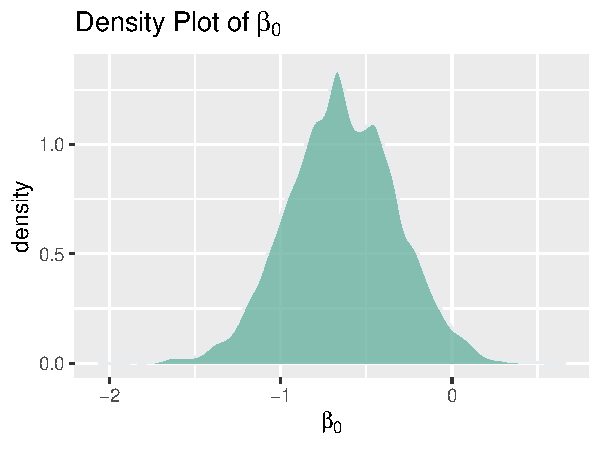
\includegraphics[width=\maxwidth]{figure/unnamed-chunk-29-1} 
\begin{kframe}\begin{alltt}
\hlkwd{ggplot}\hlstd{(}\hlkwc{data} \hlstd{= Post.Samp2.1,}\hlkwd{aes}\hlstd{(}\hlkwc{x}\hlstd{=b1))} \hlopt{+}
  \hlkwd{geom_density}\hlstd{(}\hlkwc{fill}\hlstd{=}\hlstr{"#69b3a2"}\hlstd{,} \hlkwc{color}\hlstd{=}\hlstr{"#e9ecef"}\hlstd{,} \hlkwc{alpha}\hlstd{=}\hlnum{0.8}\hlstd{)} \hlopt{+}
  \hlkwd{labs}\hlstd{(}\hlkwc{title} \hlstd{=} \hlkwd{bquote}\hlstd{(}\hlstr{"Density Plot of"} \hlopt{~} \hlstd{beta[}\hlnum{1}\hlstd{]),}\hlkwc{x} \hlstd{=} \hlkwd{bquote}\hlstd{(beta[}\hlnum{1}\hlstd{]))}
\end{alltt}
\end{kframe}
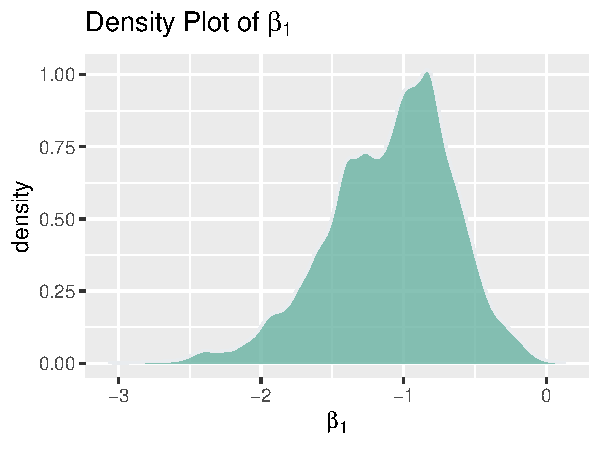
\includegraphics[width=\maxwidth]{figure/unnamed-chunk-29-2} 
\end{knitrout}
\par\end{center}

\begin{center}
\begin{knitrout}
\definecolor{shadecolor}{rgb}{0.969, 0.969, 0.969}\color{fgcolor}\begin{kframe}
\begin{alltt}
\hlcom{# plotting the mean cumulatively w.r.t sample size}
\hlstd{b0.mean.cum} \hlkwb{<-} \hlkwd{cumsum}\hlstd{(Post.Samp1}\hlopt{$}\hlstd{b0)}\hlopt{/}\hlstd{(}\hlnum{1}\hlopt{:}\hlkwd{nrow}\hlstd{(Post.Samp1))}
\hlstd{b1.mean.cum} \hlkwb{<-} \hlkwd{cumsum}\hlstd{(Post.Samp1}\hlopt{$}\hlstd{b1)}\hlopt{/}\hlstd{(}\hlnum{1}\hlopt{:}\hlkwd{nrow}\hlstd{(Post.Samp1))}

\hlcom{# plot of means with increasing sample size}
\hlkwd{plot}\hlstd{(b0.mean.cum,}\hlkwc{type} \hlstd{=} \hlstr{"l"}\hlstd{)}
\end{alltt}
\end{kframe}
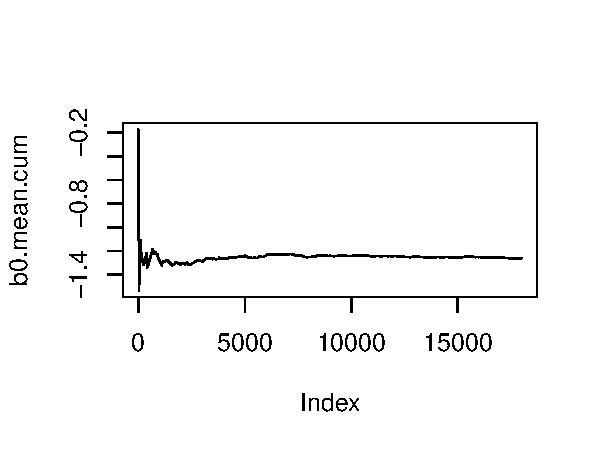
\includegraphics[width=\maxwidth]{figure/unnamed-chunk-30-1} 
\begin{kframe}\begin{alltt}
\hlkwd{plot}\hlstd{(b1.mean.cum,}\hlkwc{type} \hlstd{=} \hlstr{"l"}\hlstd{)}
\end{alltt}
\end{kframe}
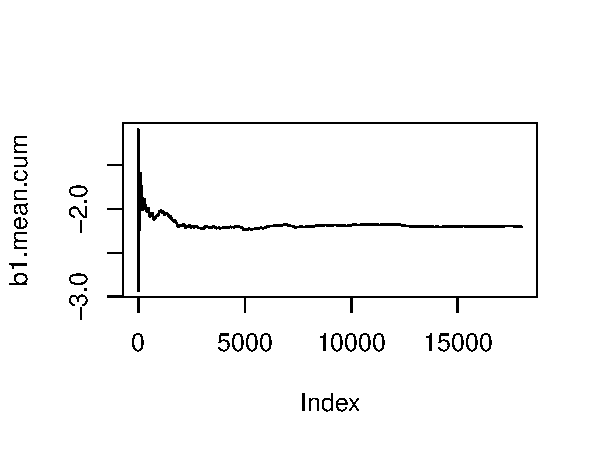
\includegraphics[width=\maxwidth]{figure/unnamed-chunk-30-2} 
\end{knitrout}
\par\end{center}

\begin{center}
\begin{knitrout}
\definecolor{shadecolor}{rgb}{0.969, 0.969, 0.969}\color{fgcolor}\begin{kframe}
\begin{alltt}
\hlcom{# Joint posterior density}
\hlkwd{library}\hlstd{(ggplot2)}

\hlcom{# b0,b1}
\hlkwd{ggplot}\hlstd{(Post.Samp2.1,} \hlkwd{aes}\hlstd{(}\hlkwc{x} \hlstd{= b0,} \hlkwc{y} \hlstd{= b1,} \hlkwc{fill} \hlstd{= ..level..))} \hlopt{+}
  \hlkwd{stat_density_2d}\hlstd{(}\hlkwc{geom} \hlstd{=} \hlstr{"polygon"}\hlstd{)} \hlopt{+}
  \hlkwd{labs}\hlstd{(}\hlkwc{title} \hlstd{=} \hlkwd{bquote}\hlstd{(}\hlstr{"Joint Density of"} \hlopt{~} \hlstd{beta[}\hlnum{0}\hlstd{]} \hlopt{~} \hlstr{"&"} \hlopt{~} \hlstd{beta[}\hlnum{1}\hlstd{]),}
\hlkwc{x} \hlstd{=} \hlkwd{bquote}\hlstd{(beta[}\hlnum{0}\hlstd{]),} \hlkwc{y} \hlstd{=} \hlkwd{bquote}\hlstd{(beta[}\hlnum{1}\hlstd{]))}
\end{alltt}
\end{kframe}
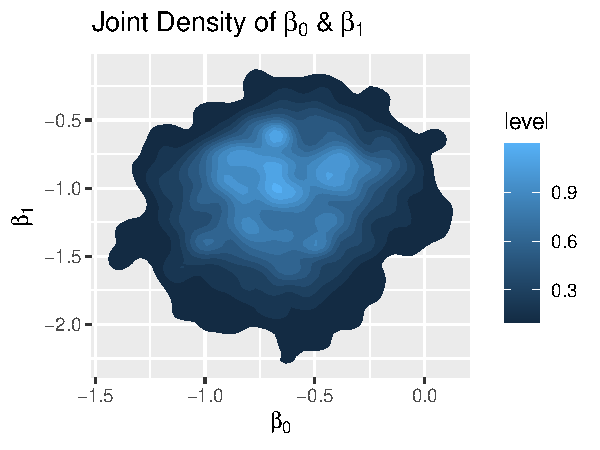
\includegraphics[width=\maxwidth]{figure/unnamed-chunk-31-1} 
\end{knitrout}
\par\end{center}

\begin{center}
\begin{knitrout}
\definecolor{shadecolor}{rgb}{0.969, 0.969, 0.969}\color{fgcolor}\begin{kframe}
\begin{alltt}
\hlcom{# Plotting the probability}
\hlstd{Post.Prob2.1} \hlkwb{<-} \hlkwa{function}\hlstd{(}\hlkwc{x.point}\hlstd{)}
\hlstd{\{}
  \hlstd{x.norm} \hlkwb{=} \hlkwa{NULL}
  \hlstd{x.norm[}\hlnum{1}\hlstd{]} \hlkwb{=} \hlstd{(x.point[}\hlnum{1}\hlstd{]} \hlopt{-} \hlkwd{mean}\hlstd{(Challeng}\hlopt{$}\hlstd{temp))}\hlopt{/}\hlkwd{sd}\hlstd{(Challeng}\hlopt{$}\hlstd{temp)}
  \hlstd{x.norm[}\hlnum{2}\hlstd{]} \hlkwb{=} \hlstd{(x.point[}\hlnum{2}\hlstd{]} \hlopt{-} \hlkwd{mean}\hlstd{(Challeng}\hlopt{$}\hlstd{pres))}\hlopt{/}\hlkwd{sd}\hlstd{(Challeng}\hlopt{$}\hlstd{pres)}
  \hlstd{x_val} \hlkwb{=} \hlkwd{matrix}\hlstd{(}\hlkwd{c}\hlstd{(}\hlnum{1}\hlstd{,x.norm),}\hlkwc{nrow} \hlstd{=} \hlnum{1}\hlstd{)}
  \hlstd{y_reg} \hlkwb{=} \hlstd{x_val}\hlopt\hlkwd{t}\hlstd{(Post.Samp2.1)}
  \hlstd{y_reg} \hlkwb{=} \hlkwd{as.vector}\hlstd{(y_reg)}
  \hlstd{Pi.Posterior} \hlkwb{<-} \hlkwd{pnorm}\hlstd{(}\hlkwc{q} \hlstd{= y_reg)}
  \hlkwd{return}\hlstd{(}\hlkwd{list}\hlstd{(}\hlstr{"samples"} \hlstd{= Pi.Posterior,}\hlstr{"post.mean"} \hlstd{=} \hlkwd{mean}\hlstd{(Pi.Posterior)))}
\hlstd{\}}

\hlstd{temp.vals} \hlkwb{<-} \hlnum{40}\hlopt{:}\hlnum{100}
\hlstd{post.mean.vec} \hlkwb{<-} \hlkwd{sapply}\hlstd{(temp.vals,} \hlkwa{function}\hlstd{(}\hlkwc{x}\hlstd{)\{}\hlkwd{return}\hlstd{(}\hlkwd{Post.Prob2.1}\hlstd{(}\hlkwc{x.point} \hlstd{=} \hlkwd{c}\hlstd{(x,}\hlnum{50}\hlstd{))}\hlopt{$}\hlstd{post.mean)\})}
\hlstd{post.mean} \hlkwb{<-} \hlkwd{data.frame}\hlstd{(}\hlstr{"x"} \hlstd{= temp.vals,}\hlstr{"post.mean"} \hlstd{= post.mean.vec)}
\hlstd{sd} \hlkwb{<-} \hlkwd{sapply}\hlstd{(temp.vals,} \hlkwa{function}\hlstd{(}\hlkwc{x}\hlstd{)\{}\hlkwd{return}\hlstd{(}\hlkwd{sd}\hlstd{(}\hlkwd{Post.Prob2.1}\hlstd{(}\hlkwc{x.point} \hlstd{=} \hlkwd{c}\hlstd{(x,}\hlnum{50}\hlstd{))}\hlopt{$}\hlstd{samples))\})}
\hlkwd{ggplot}\hlstd{(post.mean)} \hlopt{+}
  \hlkwd{geom_line}\hlstd{(}\hlkwd{aes}\hlstd{(}\hlkwc{x} \hlstd{= temp.vals,}\hlkwc{y} \hlstd{= post.mean.vec))} \hlopt{+}
  \hlkwd{ylim}\hlstd{(}\hlkwd{c}\hlstd{(}\hlnum{0}\hlstd{,}\hlnum{1}\hlstd{))} \hlopt{+}
  \hlkwd{geom_point}\hlstd{(}\hlkwc{data} \hlstd{= Challeng,}\hlkwd{aes}\hlstd{(}\hlkwc{x} \hlstd{= temp,}\hlkwc{y} \hlstd{= Datas}\hlopt{$}\hlstd{Datas.fail))} \hlopt{+}
  \hlkwd{geom_errorbar}\hlstd{(}\hlkwd{aes}\hlstd{(}\hlkwc{x} \hlstd{= temp.vals,}\hlkwc{ymin} \hlstd{= post.mean.vec} \hlopt{-} \hlstd{sd}\hlopt{/}\hlnum{2}\hlstd{,}\hlkwc{ymax} \hlstd{= post.mean.vec} \hlopt{+} \hlstd{sd}\hlopt{/}\hlnum{2}\hlstd{),} \hlkwc{linewidth}\hlstd{=}\hlnum{0.4}\hlstd{,} \hlkwc{colour}\hlstd{=}\hlstr{"blue"}\hlstd{,} \hlkwc{alpha}\hlstd{=}\hlnum{0.9}\hlstd{,} \hlkwc{size}\hlstd{=}\hlnum{1.3}\hlstd{)} \hlopt{+}
  \hlkwd{labs}\hlstd{(}\hlkwc{title} \hlstd{=} \hlstr{"Posterior Mean of Failure Probability with Error Bars"}\hlstd{,}\hlkwc{xlab} \hlstd{=} \hlstr{"Tempareture"}\hlstd{,}\hlkwc{ylab} \hlstd{=} \hlstr{"Posterior Mean"}\hlstd{)}
\end{alltt}
\end{kframe}
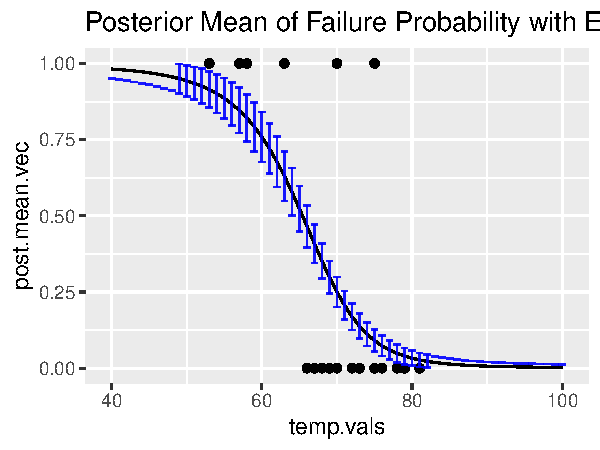
\includegraphics[width=\maxwidth]{figure/unnamed-chunk-32-1} 
\end{knitrout}
\par\end{center}

We can see that the results seem to in alignment with the data and
quite similar to what we got in case of the logistic models.

Lastly, we see how the failure probability changes with changing tempareture.
\begin{center}
\begin{knitrout}
\definecolor{shadecolor}{rgb}{0.969, 0.969, 0.969}\color{fgcolor}\begin{kframe}
\begin{alltt}
\hlstd{x.point1} \hlkwb{=} \hlkwd{c}\hlstd{(}\hlnum{75}\hlstd{,}\hlnum{50}\hlstd{)}
\hlstd{Samples.PRob} \hlkwb{<-} \hlkwd{Post.Prob2.1}\hlstd{(}\hlkwc{x.point} \hlstd{= x.point1)}\hlopt{$}\hlstd{samples}
\hlstd{Samples.PRob} \hlkwb{<-} \hlkwd{as.data.frame}\hlstd{(Samples.PRob)}
\hlkwd{ggplot}\hlstd{(}\hlkwc{data} \hlstd{= Samples.PRob,}\hlkwd{aes}\hlstd{(Samples.PRob))} \hlopt{+}
  \hlkwd{geom_density}\hlstd{(}\hlkwc{fill}\hlstd{=}\hlstr{"#69b3a2"}\hlstd{,} \hlkwc{color}\hlstd{=}\hlstr{"#e9ecef"}\hlstd{,} \hlkwc{alpha}\hlstd{=}\hlnum{0.8}\hlstd{)} \hlopt{+}
  \hlkwd{labs}\hlstd{(}\hlkwc{title} \hlstd{=} \hlkwd{bquote}\hlstd{(}\hlstr{"Posterior Density Plot of"} \hlopt{~} \hlkwd{pi}\hlstd{(X)),}
\hlkwc{x} \hlstd{=} \hlkwd{bquote}\hlstd{(}\hlstr{"Temp = "} \hlopt{~} \hlkwd{.}\hlstd{(x.point1[}\hlnum{1}\hlstd{])} \hlopt{~} \hlstr{",Pres = "} \hlopt{~} \hlkwd{.}\hlstd{(x.point1[}\hlnum{2}\hlstd{])))}
\end{alltt}
\end{kframe}
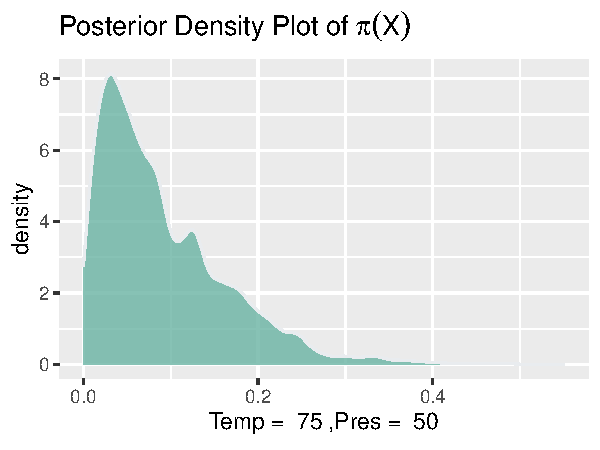
\includegraphics[width=\maxwidth]{figure/unnamed-chunk-33-1} 
\end{knitrout}
\par\end{center}

\begin{center}
\begin{knitrout}
\definecolor{shadecolor}{rgb}{0.969, 0.969, 0.969}\color{fgcolor}\begin{kframe}
\begin{alltt}
\hlstd{x.point1} \hlkwb{=} \hlkwd{c}\hlstd{(}\hlnum{60}\hlstd{,}\hlnum{50}\hlstd{)}
\hlstd{Samples.PRob} \hlkwb{<-} \hlkwd{Post.Prob2.1}\hlstd{(}\hlkwc{x.point} \hlstd{= x.point1)}\hlopt{$}\hlstd{samples}
\hlstd{Samples.PRob} \hlkwb{<-} \hlkwd{as.data.frame}\hlstd{(Samples.PRob)}
\hlkwd{ggplot}\hlstd{(}\hlkwc{data} \hlstd{= Samples.PRob,}\hlkwd{aes}\hlstd{(Samples.PRob))} \hlopt{+}
  \hlkwd{geom_density}\hlstd{(}\hlkwc{fill}\hlstd{=}\hlstr{"#69b3a2"}\hlstd{,} \hlkwc{color}\hlstd{=}\hlstr{"#e9ecef"}\hlstd{,} \hlkwc{alpha}\hlstd{=}\hlnum{0.8}\hlstd{)} \hlopt{+}
  \hlkwd{labs}\hlstd{(}\hlkwc{title} \hlstd{=} \hlkwd{bquote}\hlstd{(}\hlstr{"Posterior Density Plot of"} \hlopt{~} \hlkwd{pi}\hlstd{(X)),}
\hlkwc{x} \hlstd{=} \hlkwd{bquote}\hlstd{(}\hlstr{"Temp = "} \hlopt{~} \hlkwd{.}\hlstd{(x.point1[}\hlnum{1}\hlstd{])} \hlopt{~} \hlstr{",Pres = "} \hlopt{~} \hlkwd{.}\hlstd{(x.point1[}\hlnum{2}\hlstd{])))}
\end{alltt}
\end{kframe}
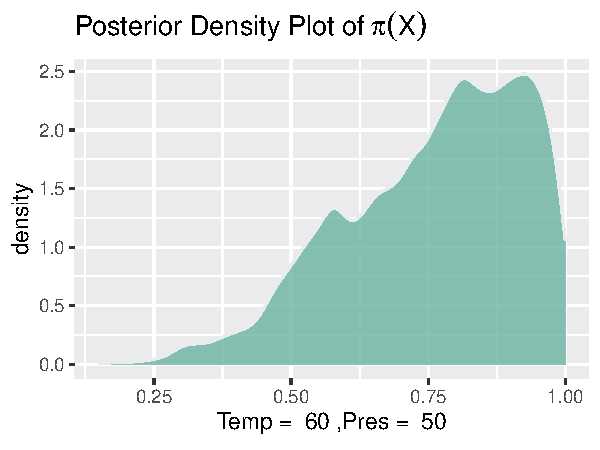
\includegraphics[width=\maxwidth]{figure/unnamed-chunk-34-1} 
\end{knitrout}
\par\end{center}

\begin{center}
\begin{knitrout}
\definecolor{shadecolor}{rgb}{0.969, 0.969, 0.969}\color{fgcolor}\begin{kframe}
\begin{alltt}
\hlstd{x.point1} \hlkwb{=} \hlkwd{c}\hlstd{(}\hlnum{45}\hlstd{,}\hlnum{50}\hlstd{)}
\hlstd{Samples.PRob} \hlkwb{<-} \hlkwd{Post.Prob2.1}\hlstd{(}\hlkwc{x.point} \hlstd{= x.point1)}\hlopt{$}\hlstd{samples}
\hlstd{Samples.PRob} \hlkwb{<-} \hlkwd{as.data.frame}\hlstd{(Samples.PRob)}
\hlkwd{ggplot}\hlstd{(}\hlkwc{data} \hlstd{= Samples.PRob,}\hlkwd{aes}\hlstd{(Samples.PRob))} \hlopt{+}
  \hlkwd{geom_density}\hlstd{(}\hlkwc{fill}\hlstd{=}\hlstr{"#69b3a2"}\hlstd{,} \hlkwc{color}\hlstd{=}\hlstr{"#e9ecef"}\hlstd{,} \hlkwc{alpha}\hlstd{=}\hlnum{0.8}\hlstd{)} \hlopt{+}
  \hlkwd{labs}\hlstd{(}\hlkwc{title} \hlstd{=} \hlkwd{bquote}\hlstd{(}\hlstr{"Posterior Density Plot of"} \hlopt{~} \hlkwd{pi}\hlstd{(X)),}
\hlkwc{x} \hlstd{=} \hlkwd{bquote}\hlstd{(}\hlstr{"Temp = "} \hlopt{~} \hlkwd{.}\hlstd{(x.point1[}\hlnum{1}\hlstd{])} \hlopt{~} \hlstr{",Pres = "} \hlopt{~} \hlkwd{.}\hlstd{(x.point1[}\hlnum{2}\hlstd{])))}
\end{alltt}
\end{kframe}
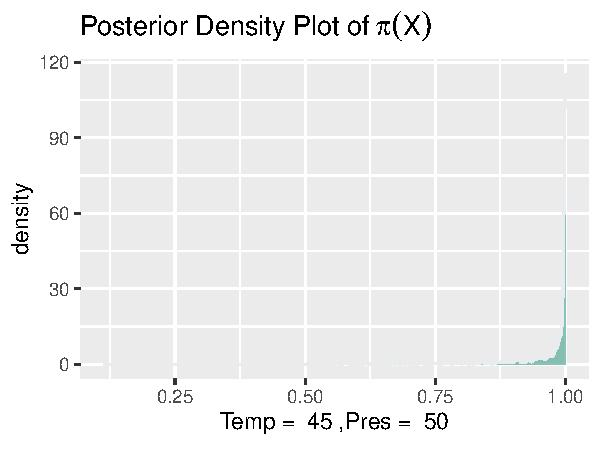
\includegraphics[width=\maxwidth]{figure/unnamed-chunk-35-1} 
\end{knitrout}
\par\end{center}

We can see here, also the results obtained are quite satisfactory.
\author{\pagebreak}

\section*{Model Comparison}

\subsection*{Using Naive Monte Carlo}

Finally we compare between these two bayesian models one with logistic
link and one with probit link function. We can use bayes factor to
compare between them. Here, our hypothesis are :-

\begin{align*}
M_{0}: & \text{The model involving logit link is as good as that}\\
 & \text{involving the probit link.}\\
M_{1}: & \text{These two models are not same but one is better}\\
 & \text{than the other.}
\end{align*}
 we use the bayes factor here also defined as 
\[
BF_{10}=\frac{m_{1}\left(\boldsymbol{X,y}\right)}{m_{0}\left(\boldsymbol{X,y}\right)}
\]
 where, $m_{i}\left(\boldsymbol{X,y}\right)=\int f_{i}\left(\boldsymbol{y}|\boldsymbol{\beta},\boldsymbol{x}\right)\pi_{i}\left(\boldsymbol{\beta}\right)d\boldsymbol{\beta}$
for $i=1,2$. We use naive monte carlo method to calculate the values
of the integrals through a numerical method using samples drawn from
prior distribution. Here is the code for the computation and we obtain
the approx value of bayes factor.

\begin{knitrout}
\definecolor{shadecolor}{rgb}{0.969, 0.969, 0.969}\color{fgcolor}\begin{kframe}
\begin{alltt}
\hlcom{# Comparison using Bayes Factor}
\hlstd{m2.1} \hlkwb{<-} \hlkwa{function}\hlstd{(}\hlkwc{X}\hlstd{,}\hlkwc{y}\hlstd{,}\hlkwc{lambda} \hlstd{=} \hlnum{0.0001}\hlstd{,}\hlkwc{N} \hlstd{=} \hlnum{10}\hlopt{^}\hlnum{3}\hlstd{,}\hlkwc{null} \hlstd{=} \hlnum{TRUE}\hlstd{,}\hlkwc{Fac} \hlstd{=} \hlnum{10}\hlopt{^}\hlnum{3}\hlstd{,}\hlkwc{param} \hlstd{=} \hlnum{1}\hlstd{)}
\hlstd{\{}
  \hlstd{beta} \hlkwb{=} \hlkwd{c}\hlstd{()}
  \hlstd{Total} \hlkwb{=} \hlnum{0}
  \hlstd{X} \hlkwb{=} \hlkwd{cbind}\hlstd{(}\hlkwd{rep}\hlstd{(}\hlnum{1}\hlstd{,}\hlkwd{nrow}\hlstd{(X)),X)}
  \hlkwa{for}\hlstd{(i} \hlkwa{in} \hlnum{1}\hlopt{:}\hlstd{N)}
  \hlstd{\{}
    \hlstd{beta[}\hlnum{1}\hlstd{]} \hlkwb{=} \hlkwd{rnorm}\hlstd{(}\hlnum{1}\hlstd{,}\hlnum{0}\hlstd{,}\hlkwc{sd} \hlstd{=} \hlnum{1}\hlopt{/}\hlstd{lambda)}
    \hlstd{beta[}\hlnum{2}\hlstd{]} \hlkwb{=} \hlkwd{rnorm}\hlstd{(}\hlnum{1}\hlstd{,}\hlnum{0}\hlstd{,}\hlkwc{sd} \hlstd{=} \hlnum{1}\hlopt{/}\hlstd{lambda)}
    \hlstd{beta[}\hlnum{3}\hlstd{]} \hlkwb{=} \hlkwd{rnorm}\hlstd{(}\hlnum{1}\hlstd{,}\hlnum{0}\hlstd{,}\hlkwc{sd} \hlstd{=} \hlnum{1}\hlopt{/}\hlstd{lambda)}

    \hlkwa{if}\hlstd{(null)\{}
      \hlstd{beta[param]} \hlkwb{=} \hlnum{0}
    \hlstd{\}}

    \hlstd{beta} \hlkwb{=} \hlkwd{matrix}\hlstd{(beta,}\hlkwc{byrow} \hlstd{=} \hlnum{TRUE}\hlstd{,}\hlkwc{nrow} \hlstd{=} \hlnum{1}\hlstd{)}
    \hlstd{b} \hlkwb{=} \hlkwd{exp}\hlstd{(y}\hlopt{*}\hlstd{(beta}\hlopt\hlkwd{t}\hlstd{(X)))}
    \hlstd{c} \hlkwb{=} \hlkwd{exp}\hlstd{(beta}\hlopt\hlkwd{t}\hlstd{(X))}
    \hlstd{M} \hlkwb{=} \hlstd{Fac}\hlopt{*}\hlkwd{prod}\hlstd{(b}\hlopt{/}\hlstd{(}\hlnum{1}\hlopt{+}\hlstd{c))}
    \hlstd{Total} \hlkwb{=} \hlstd{M} \hlopt{+} \hlstd{Total}
  \hlstd{\}}
  \hlkwd{return}\hlstd{(Total}\hlopt{/}\hlstd{N)}
\hlstd{\}}

\hlcom{# New model}
\hlstd{m2.2} \hlkwb{<-} \hlkwa{function}\hlstd{(}\hlkwc{X}\hlstd{,}\hlkwc{y}\hlstd{,}\hlkwc{lambda} \hlstd{=} \hlnum{0.0001}\hlstd{,}\hlkwc{N} \hlstd{=} \hlnum{10}\hlopt{^}\hlnum{3}\hlstd{,}\hlkwc{null} \hlstd{=} \hlnum{TRUE}\hlstd{,}\hlkwc{Fac} \hlstd{=} \hlnum{10}\hlopt{^}\hlnum{3}\hlstd{,}\hlkwc{param} \hlstd{=} \hlnum{1}\hlstd{)}
\hlstd{\{}
  \hlstd{beta} \hlkwb{=} \hlkwd{c}\hlstd{()}
  \hlstd{Total} \hlkwb{=} \hlnum{0}
  \hlstd{X} \hlkwb{=} \hlkwd{cbind}\hlstd{(}\hlkwd{rep}\hlstd{(}\hlnum{1}\hlstd{,}\hlkwd{nrow}\hlstd{(X)),X)}
  \hlkwa{for}\hlstd{(i} \hlkwa{in} \hlnum{1}\hlopt{:}\hlstd{N)}
  \hlstd{\{}
    \hlstd{beta[}\hlnum{1}\hlstd{]} \hlkwb{=} \hlkwd{rnorm}\hlstd{(}\hlnum{1}\hlstd{,}\hlnum{0}\hlstd{,}\hlkwc{sd} \hlstd{=} \hlnum{1}\hlopt{/}\hlstd{lambda)}
    \hlstd{beta[}\hlnum{2}\hlstd{]} \hlkwb{=} \hlkwd{rnorm}\hlstd{(}\hlnum{1}\hlstd{,}\hlnum{0}\hlstd{,}\hlkwc{sd} \hlstd{=} \hlnum{1}\hlopt{/}\hlstd{lambda)}
    \hlstd{beta[}\hlnum{3}\hlstd{]} \hlkwb{=} \hlkwd{rnorm}\hlstd{(}\hlnum{1}\hlstd{,}\hlnum{0}\hlstd{,}\hlkwc{sd} \hlstd{=} \hlnum{1}\hlopt{/}\hlstd{lambda)}

    \hlkwa{if}\hlstd{(null)\{}
      \hlstd{beta[param]} \hlkwb{=} \hlnum{0}
    \hlstd{\}}

    \hlstd{b} \hlkwb{=} \hlkwd{pnorm}\hlstd{(}\hlkwc{q} \hlstd{= beta}\hlopt\hlkwd{t}\hlstd{(X))}
    \hlstd{c} \hlkwb{=} \hlstd{(b}\hlopt{^}\hlstd{y)}\hlopt{*}\hlstd{((}\hlnum{1}\hlopt{-}\hlstd{b)}\hlopt{^}\hlstd{(}\hlnum{1}\hlopt{-}\hlstd{y))}
    \hlstd{M} \hlkwb{=} \hlstd{Fac}\hlopt{*}\hlkwd{prod}\hlstd{(c)}

    \hlstd{Total} \hlkwb{=} \hlstd{M} \hlopt{+} \hlstd{Total}
  \hlstd{\}}
  \hlkwd{return}\hlstd{(Total}\hlopt{/}\hlstd{N)}
\hlstd{\}}

\hlkwd{set.seed}\hlstd{(}\hlnum{1000}\hlstd{)}
\hlstd{a} \hlkwb{=} \hlkwd{m2.1}\hlstd{(}\hlkwc{X} \hlstd{= Datas[,}\hlnum{1}\hlopt{:}\hlnum{2}\hlstd{],}\hlkwc{y} \hlstd{= Datas}\hlopt{$}\hlstd{Datas.fail,}\hlkwc{N} \hlstd{=} \hlnum{10}\hlopt{^}\hlnum{4}\hlstd{,}
\hlkwc{lambda} \hlstd{=} \hlnum{0.1}\hlstd{,}\hlkwc{null} \hlstd{=} \hlnum{TRUE}\hlstd{,}\hlkwc{param} \hlstd{=} \hlnum{3}\hlstd{)}
\hlkwd{set.seed}\hlstd{(}\hlnum{1000}\hlstd{)}
\hlstd{b} \hlkwb{=} \hlkwd{m2.2}\hlstd{(}\hlkwc{X} \hlstd{= Datas[,}\hlnum{1}\hlopt{:}\hlnum{2}\hlstd{],}\hlkwc{y} \hlstd{= Datas}\hlopt{$}\hlstd{Datas.fail,}\hlkwc{N} \hlstd{=} \hlnum{10}\hlopt{^}\hlnum{4}\hlstd{,}
\hlkwc{lambda} \hlstd{=} \hlnum{0.1}\hlstd{,}\hlkwc{null} \hlstd{=} \hlnum{TRUE}\hlstd{,}\hlkwc{param} \hlstd{=} \hlnum{3}\hlstd{)}
\hlstd{a;b}
\end{alltt}
\begin{verbatim}
[1] 0.0001415287
[1] 3.899003e-05
\end{verbatim}
\begin{alltt}
\hlstd{BF10} \hlkwb{=} \hlstd{b}\hlopt{/}\hlstd{a}
\hlkwd{log}\hlstd{(BF10)}
\end{alltt}
\begin{verbatim}
[1] -1.289196
\end{verbatim}
\end{kframe}
\end{knitrout}

As can be seen the value is small hence, we have no evidence whatsoever
to reject the alternate hypothesis hence, we accept $H_{0}$ here.

\subsection*{Using Harmonic Mean Estimator}

Secondly, we use the harmonic estimator which utilizes the posterior
samples generated using MCMC to calculate the marginal likelihoods.
We define it as :-
\[
\widetilde{Z}_{\mathcal{M}}=\left[\frac{1}{N}\sum_{i=1}^{N}\frac{1}{f\left(\boldsymbol{X,y}|\boldsymbol{\beta}^{\left(i\right)},\mathcal{M}\right)}\right]_{\boldsymbol{\beta}^{\left(i\right)}\sim\pi\left(\boldsymbol{\beta}|\boldsymbol{X,y}\right)}^{-1}
\]

Using this we calculate $\widetilde{Z}_{\mathcal{M}_{1}}$ and $\widetilde{Z}_{\mathcal{M}_{0}}$
and calculate their ratio to evaluate approximate value of $BF_{10}$
as :-
\[
\widetilde{\text{BF}}_{10}=\frac{\widetilde{Z}_{\mathcal{M}_{1}}}{\widetilde{Z}_{\mathcal{M}_{0}}}
\]

which came around clsoe to 1 (not significantly different from 1)
and as this value is not very much significant in favour of $H_{1}$
so we accept $H_{0}$ and conclude that both the models are more or
less equivalent.

\begin{knitrout}
\definecolor{shadecolor}{rgb}{0.969, 0.969, 0.969}\color{fgcolor}\begin{kframe}
\begin{alltt}
\hlcom{# Using harmonic estimator}
\hlcom{# Logistic Model}
\hlstd{N} \hlkwb{=} \hlkwd{nrow}\hlstd{(Post.Samp2)}
\hlstd{Total} \hlkwb{=} \hlnum{0}
\hlstd{X} \hlkwb{=} \hlkwd{cbind}\hlstd{(}\hlkwd{rep}\hlstd{(}\hlnum{1}\hlstd{,}\hlkwd{nrow}\hlstd{(Datas)),Datas[,}\hlnum{1}\hlopt{:}\hlnum{2}\hlstd{]);y} \hlkwb{=} \hlstd{Datas}\hlopt{$}\hlstd{Datas.fail}
\hlstd{M1} \hlkwb{=} \hlkwa{NULL}

\hlkwa{for}\hlstd{(i} \hlkwa{in} \hlnum{1}\hlopt{:}\hlstd{N)}
\hlstd{\{}
  \hlstd{beta} \hlkwb{=} \hlstd{Post.Samp2[i,]}
  \hlstd{beta} \hlkwb{=} \hlkwd{cbind}\hlstd{(beta,}\hlnum{0}\hlstd{)}
  \hlstd{beta} \hlkwb{=} \hlkwd{as.matrix}\hlstd{(beta)}
  \hlstd{b} \hlkwb{=} \hlkwd{exp}\hlstd{(y}\hlopt{*}\hlstd{(beta}\hlopt\hlkwd{t}\hlstd{(X)))}
  \hlstd{c} \hlkwb{=} \hlkwd{exp}\hlstd{(beta}\hlopt\hlkwd{t}\hlstd{(X))}
  \hlstd{M1[i]} \hlkwb{=} \hlkwd{prod}\hlstd{(b}\hlopt{/}\hlstd{(}\hlnum{1}\hlopt{+}\hlstd{c))}
\hlstd{\}}
\hlstd{Est1} \hlkwb{=} \hlnum{1}\hlopt{/}\hlkwd{mean}\hlstd{(}\hlnum{1}\hlopt{/}\hlstd{M1)}

\hlcom{# Probit Model}
\hlstd{N} \hlkwb{=} \hlkwd{nrow}\hlstd{(Post.Samp2.1)}
\hlstd{Total} \hlkwb{=} \hlnum{0}
\hlstd{X} \hlkwb{=} \hlkwd{cbind}\hlstd{(}\hlkwd{rep}\hlstd{(}\hlnum{1}\hlstd{,}\hlkwd{nrow}\hlstd{(Datas)),Datas[,}\hlnum{1}\hlopt{:}\hlnum{2}\hlstd{]);y} \hlkwb{=} \hlstd{Datas}\hlopt{$}\hlstd{Datas.fail}
\hlstd{M2} \hlkwb{=} \hlkwa{NULL}
\hlstd{i} \hlkwb{=} \hlnum{1}
\hlkwa{for}\hlstd{(i} \hlkwa{in} \hlnum{1}\hlopt{:}\hlstd{N)}
\hlstd{\{}
  \hlstd{beta} \hlkwb{=} \hlstd{Post.Samp2.1[i,]}
  \hlstd{beta} \hlkwb{=} \hlkwd{as.matrix}\hlstd{(beta)}
  \hlstd{b} \hlkwb{=} \hlkwd{pnorm}\hlstd{(}\hlkwc{q} \hlstd{= beta}\hlopt\hlkwd{t}\hlstd{(X))}
  \hlstd{c} \hlkwb{=} \hlstd{(b}\hlopt{^}\hlstd{y)}\hlopt{*}\hlstd{((}\hlnum{1}\hlopt{-}\hlstd{b)}\hlopt{^}\hlstd{(}\hlnum{1}\hlopt{-}\hlstd{y))}
  \hlstd{M2[i]} \hlkwb{=} \hlkwd{prod}\hlstd{(c)}
\hlstd{\}}
\hlstd{Est2} \hlkwb{=} \hlnum{1}\hlopt{/}\hlkwd{mean}\hlstd{(}\hlnum{1}\hlopt{/}\hlstd{M2)}

\hlcom{## Estimated Value of Bayes Factor(10)}
\hlstd{Est1}\hlopt{/}\hlstd{Est2}
\end{alltt}
\begin{verbatim}
[1] 0.8954418
\end{verbatim}
\end{kframe}
\end{knitrout}

here also, we can clearly see the approximate value is quite close
to $1$ which signifies the same as before.
\end{document}
